

\chapter{Multiscale Methods on the Sphere}
\label{ch_mms}

In this chapter, many multiscale decompositions will be built 
based on the spherical harmonics and/or the HEALPix representation.

\section{Orthogonal Haar Wavelets on the Sphere}
\label{mrs_haar}
\index{wavelet!Haar on sphere}
\index{sphere!Haar}

The Haar wavelet transform on the sphere \citep{wave:sweldens95a} at each resolution $j$ and pixel $\bk=(k_x,k_y)$ on the sphere 
is based on a scaling function $\phi_{j,\bk}$ ($\phi_{j,\bk}(\bx) = \phi\parenth{2^{-j}(\bx-\bk)}$, where $\bx$ is the vector of 
Cartesian coordinates on the sphere, and $\phi$ is the Haar scaling function) and three Haar wavelet functions $\psi^{d}_{j,\bk}$ (see~\eqref{def_whaar1})
with $d \in\{1,2,3\}$. It uses the idea that a given pixel on the sphere at a given resolution $j$ in the HEALPix representation
is directly related to four pixels at the next resolution $j-1$.  
% For Healpix  pixelisation, resolution of the map is related 
% to the  $N_{side}$ parameter, 
% which corresponds to the square root of number of pixels in each face.
% $ N_{side} = 2^{j-1}$.  At a given resolution  $j$ we have $n_j=12 \times 4^{j-1}$ pixels with a surface size $\mu_j$. 

Noting, $\bk_0$, the pixel. The scaling function $\phi$ and three wavelet functions $\psi$ are defined by:
\begin{eqnarray}
\label{def_whaar1}
\phi_{j,\bk}(\bx) & = & \left\{  \begin{array}{ll}
1 & \textrm{if $t \in S_{j,\bk}$ }\\
0 & \textrm{otherwise}
   \end{array} \right.  \nonumber \\
\psi_{1,j+1,\bk} & = & \frac{\phi_{j,\bk_0} +\phi_{j,\bk_2}-\phi_{j,\bk_1}-\phi_{j,\bk_3} }{4}  \nonumber \\
\psi_{2,j+1,\bk} & = & \frac{\phi_{j,\bk_0} +\phi_{j,\bk_1}-\phi_{j,\bk_2}-\phi_{j,\bk_3} }{4}  \nonumber \\
\psi_{3,j+1,\bk} & = & \frac{\phi_{j,\bk_0} +\phi_{j,\bk_3}-\phi_{j,\bk_1}-\phi_{j,\bk_2} }{4}
\end{eqnarray}

% \begin{figure}[htb]
%\centering
%\includegraphics[width=10cm]{fig_haar_decomp.pdf}
%\label{fig_haar_decomp}
%\caption{On resolution to next using Haar.}
%\end{figure}

% \begin{figure*}
% \vbox{
% \centerline{
% \hbox{
% \includegraphics[angle=180,width=7cm]{haar0.pdf}
% \includegraphics[angle=180,width=7cm]{haar1.pdf}
% }}\centerline{
% \hbox{
% \includegraphics[angle=180,width=7cm]{haar2.pdf}
% \includegraphics[angle=180,width=7cm]{haar3.pdf}
% }}
% \centerline{
% \hbox{
% \includegraphics[angle=180,width=7cm]{haar4.pdf}
% \includegraphics[angle=180,width=7cm]{haar5.pdf}
% }}
% }
% \label{fig_haar_decomp2}
% \caption{Haar wavelet  coefficents.}
% \end{figure*}

Denoting $\bk_0,\bk_1,\bk_2,\bk_3$ the four pixels at scale $j$, hierarchically related to the pixel $\bk$ at scale $j+1$, 
scaling coefficients $c_{j+1,\bk}$ at scale $j+1$ are derived from those at scale $j$ by:
\begin{eqnarray}
\label{def_haar1}
c_{j+1}[\bk] &=& \frac{1}{4} \sum_{d=0}^3 c_{j} [\bk_d],
\end{eqnarray}
and wavelet coefficients at scale $j+1$ from coefficients at scale $j$ by:
\begin{eqnarray}
\label{def_haar2}
w^{1}_{j+1} [\bk] &=& \frac{1}{4} (c_{j}[\bk_0]+c_{j} [\bk_2] - c_{j} [\bk_1]-c_{j}[\bk_3])  \nonumber  \\
w^{2}_{j+1} [\bk] &=& \frac{1}{4} (c_{j}[\bk_0]+c_{j} [\bk_1] - c_{j} [\bk_2]-c_{j}[\bk_3])  \nonumber  \\
w^{3}_{j+1} [\bk] &=& \frac{1}{4} (c_{j}[\bk_0]+c_{j} [\bk_3] - c_{j} [\bk_1]-c_{j}[\bk_2]) .
\end{eqnarray}

% Fig. \ref{fig_haar_decomp} shows the calculation scheme of haar coefficients, from one resolution to the next. 
% Haar wavelet coefficients for the astronomical WMAP data set are shown in Fig. \ref{fig_haar_decomp2}.

The Haar wavelet transform on the sphere is orthogonal and its reconstruction is exact. The inverse transformation is obtained by:
\begin{eqnarray}
\label{def_recons_haar}
c_0[\bx] = \sum_{\bk}  c_{J}[\bk]  \phi_{J,\bk}(\bx) + \sum_{j=1}^{J} \sum_{d=1}^3 \sum_{\bk} w^{d}_{j}[\bk]  \psi^d_{j}(\bx) .
\end{eqnarray}

This transform is very fast but its interest is relatively limited. Indeed, it is not rotation invariant, and more importantly 
the Haar wavelet shape is not well adapted for most applications, because of the non-regular shape of the wavelet function.


% ===============================================

\section{Continuous Wavelets on the Sphere}

\subsection{Stereoscopic Projection}
\label{chap_mex_hat}

\index{wavelet!axisymmetrical wavelets}
\index{wavelet!stereoscopic projection}

\begin{figure}[htb]
\centering
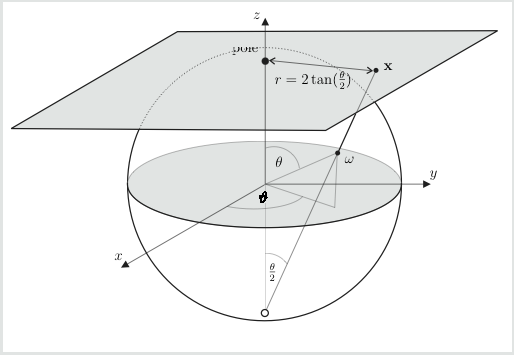
\includegraphics[width=15cm]{proj_stereo_inverse.pdf}
\caption{Inverse stereographic projections of a radial function from plane to the sphere.}
\label{figprojstereo_direct}
\end{figure}

In order to have more choice to design the wavelet function, we may want to use wavelets defined for regular 2D images to the sphere.
This is possible by using inverse stereographic projections of radial wavelet functions such the Mexican hat \citep{wave:cayon01}.
Defining the stereographic projection operator, $\bR: {\bf t} \mapsto \ {\boldsymbol \omega}$, with ${\boldsymbol \omega} = (\theta(r),\vartheta)$, 
$\theta(r) = 2 \arctan(r/2)$, the radial wavelets $\psi_{\mathrm{plane}}$ can be projected on the sphere by a unique rotation, 
${\boldsymbol \omega}_0 =(\theta_0,\vartheta_0)$, respectively around the two axes $O_y$ and $O_z$. Fig.~\ref{figprojstereo_direct} shows 
the projection of radial functions from the plane to the sphere. 
 
The convolution on the sphere between a radial wavelet function $\psi(\theta)$ and a function $f({\boldsymbol \omega})$ is:
 \begin{eqnarray}
\label{convol_sph}
(\psi \ast f)(\theta,\vartheta)= \int_{S^2} \psi_{\mathrm{plane}}^* (\bR^{-1}  {\boldsymbol \omega}) f({\boldsymbol \omega}) d{\boldsymbol \omega} .
\end{eqnarray}

Such wavelets are axisymmetric by construction. This property can be used to derive fast transformation algorithms using spherical harmonics.
Indeed spherical harmonics coefficients $\hat{\psi}[l,m]$ of the wavelet function $\psi$ on the sphere are equal to zero when $m \neq 0$, 
and by the Funk-Hecke theorem, the convolution can be written using spherical harmonics by:
\begin{eqnarray}
\label{convol_sph_harm}
(\psi \ast f)(\theta,\vartheta)  =  \sum_{l=0}^{\infty} \sum_{m=-l}^{l} \sqrt{\frac{2l+1}{4\pi} }\hat{f}[l,m] \hat{ \psi}[l,0] Y_{lm}(\theta,\vartheta) ~.
\end{eqnarray}
where $\hat{f}[l,m]$ are the spherical harmonics coefficients of the function $f$,\\ 
i.e. $f = \sum_{l=0}^{\infty}\sum_{m=-l}^{l} \hat{f}[l,m] Y_{lm}$ and similary for $\hat{\psi}$.

Classical wavelet dilations can also be derived on the sphere using the dilation operator $\mathscr{D}_a$ by a factor $a > 0$ \citep{wiaux07}:
\begin{eqnarray}
\label{proj_stereo}
\mathscr{D}_a(f)({\boldsymbol \omega}) = \chi_a^{1/2} (a,\theta)  f(D^{-1}_a {\boldsymbol \omega}) ,
\end{eqnarray}
where $D_a(\theta,\vartheta)=(\theta_a(\theta),\vartheta)$ with the linear relation $\tan\theta_a(\theta)/2=a\tan\theta/2$, 
and $D_a$ is the dilation operator that maps a sphere without its South pole on itself. $\chi_a^{1/2}(a,\theta)$ is a norm 
preservation term (i.e. $\mathscr{D}_a$ is unitary):
\begin{eqnarray}
\label{def_lambda}
\chi_a^{1/2}(a,\theta) = a^{-1}[1+\tan^2(\theta/2)]/[1+a^{-2}\tan^2(\theta/2)] ~.
\end{eqnarray}

% \begin{figure*}
% \centering
% \includegraphics[width=9cm]{proj_stereo.pdf}
% \caption{Projection st\'er\'eographique inverse sur la sphere.}
% \label{figprojstereo}
% \end{figure*}

\subsection{Mexican Hat Wavelet} 

\index{sphere!mexican hat}
\index{Mexican hat!on sphere}

\begin{figure}[htb]
\vbox{
\centerline{
\hbox{
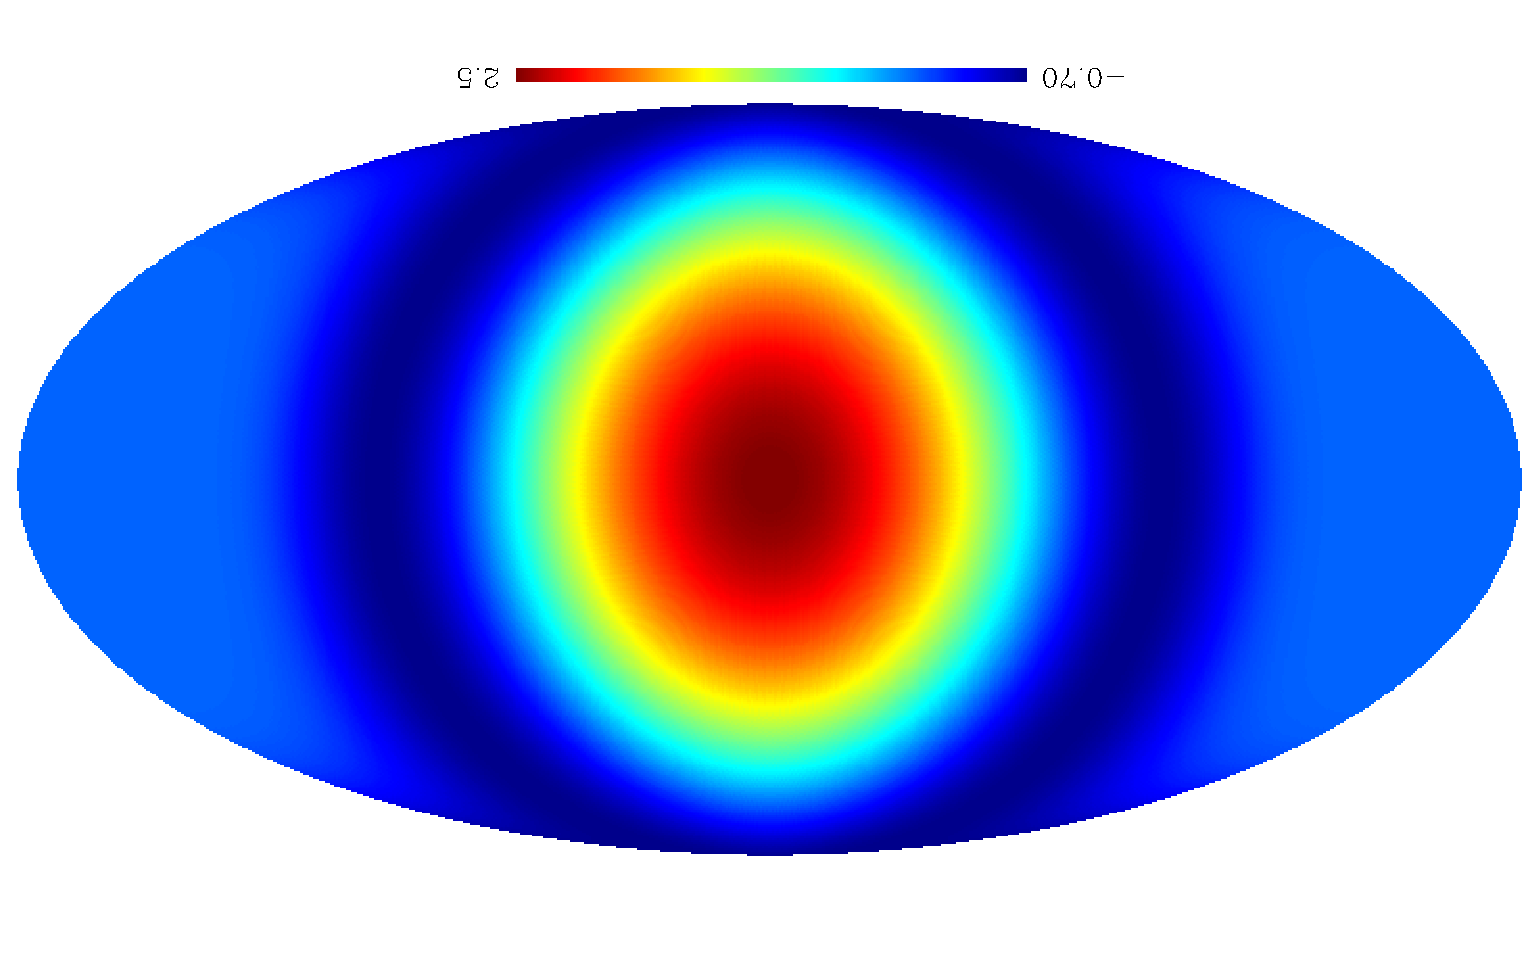
\includegraphics[angle=180,width=7.9cm]{wav_mex_hat_0.pdf}
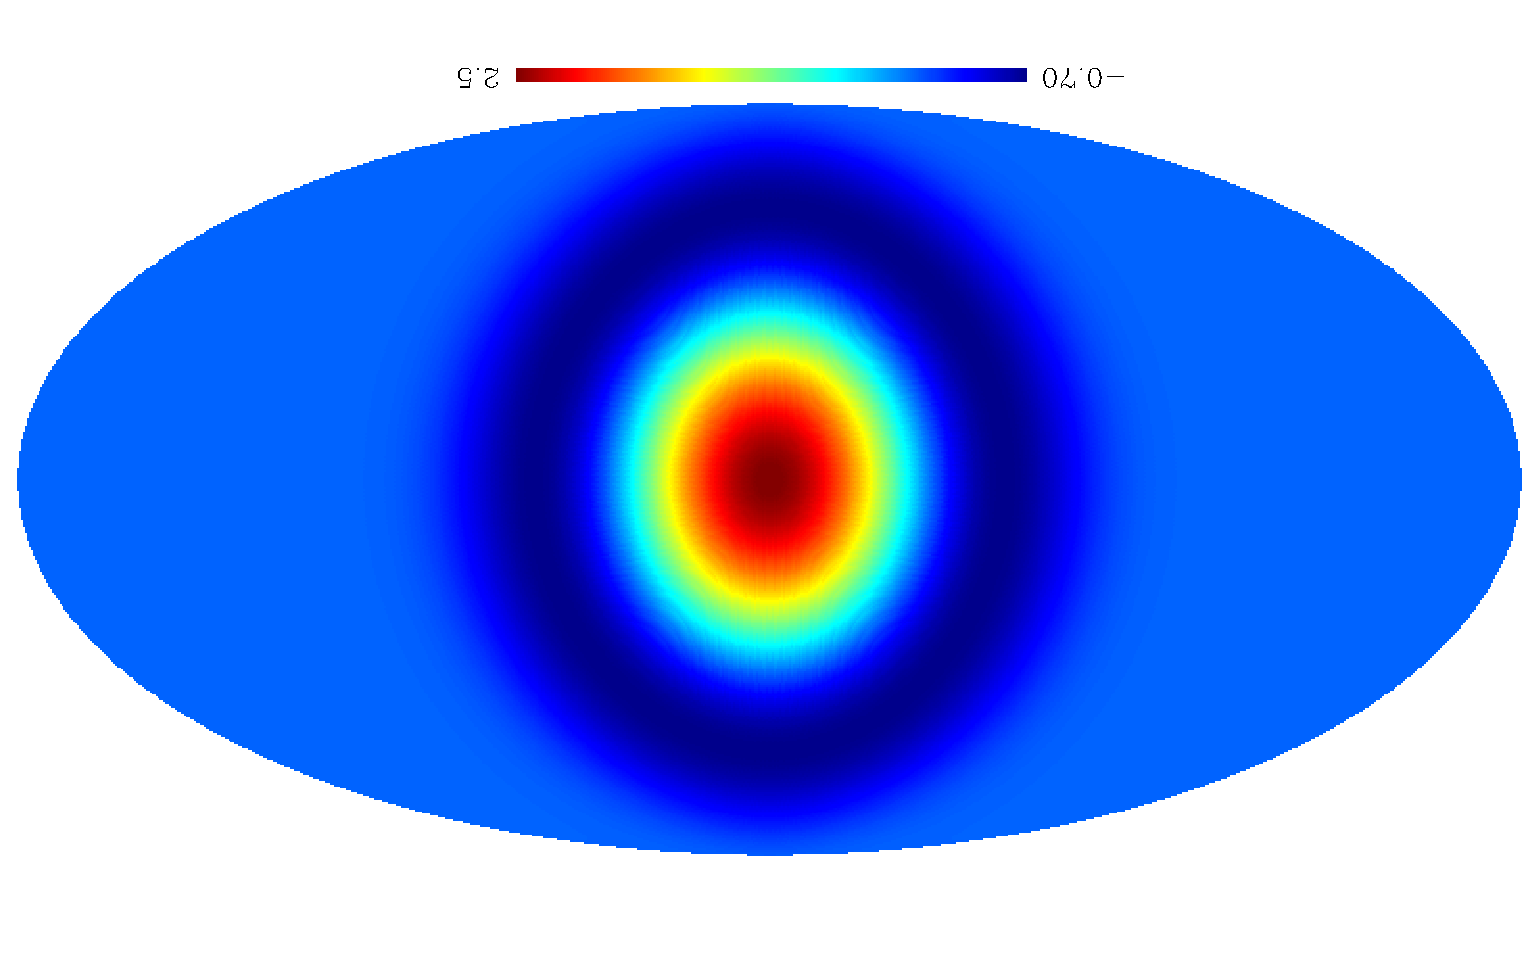
\includegraphics[angle=180,width=7.9cm]{wav_mex_hat_1.pdf}
}}\centerline{
\hbox{
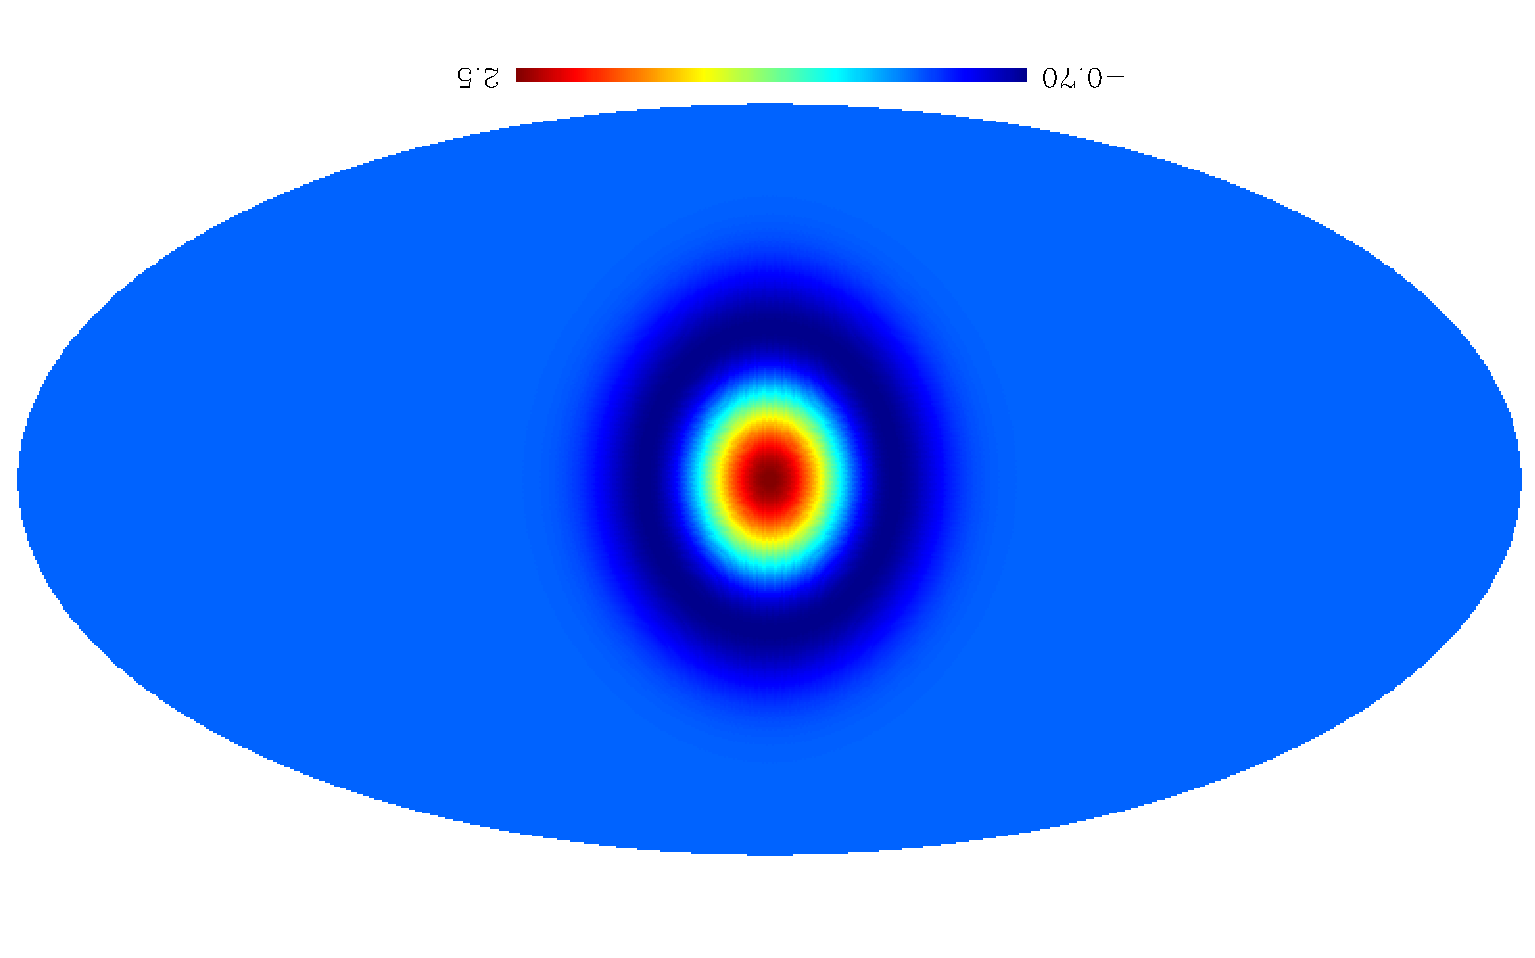
\includegraphics[angle=180,width=7.9cm]{wav_mex_hat_2.pdf}
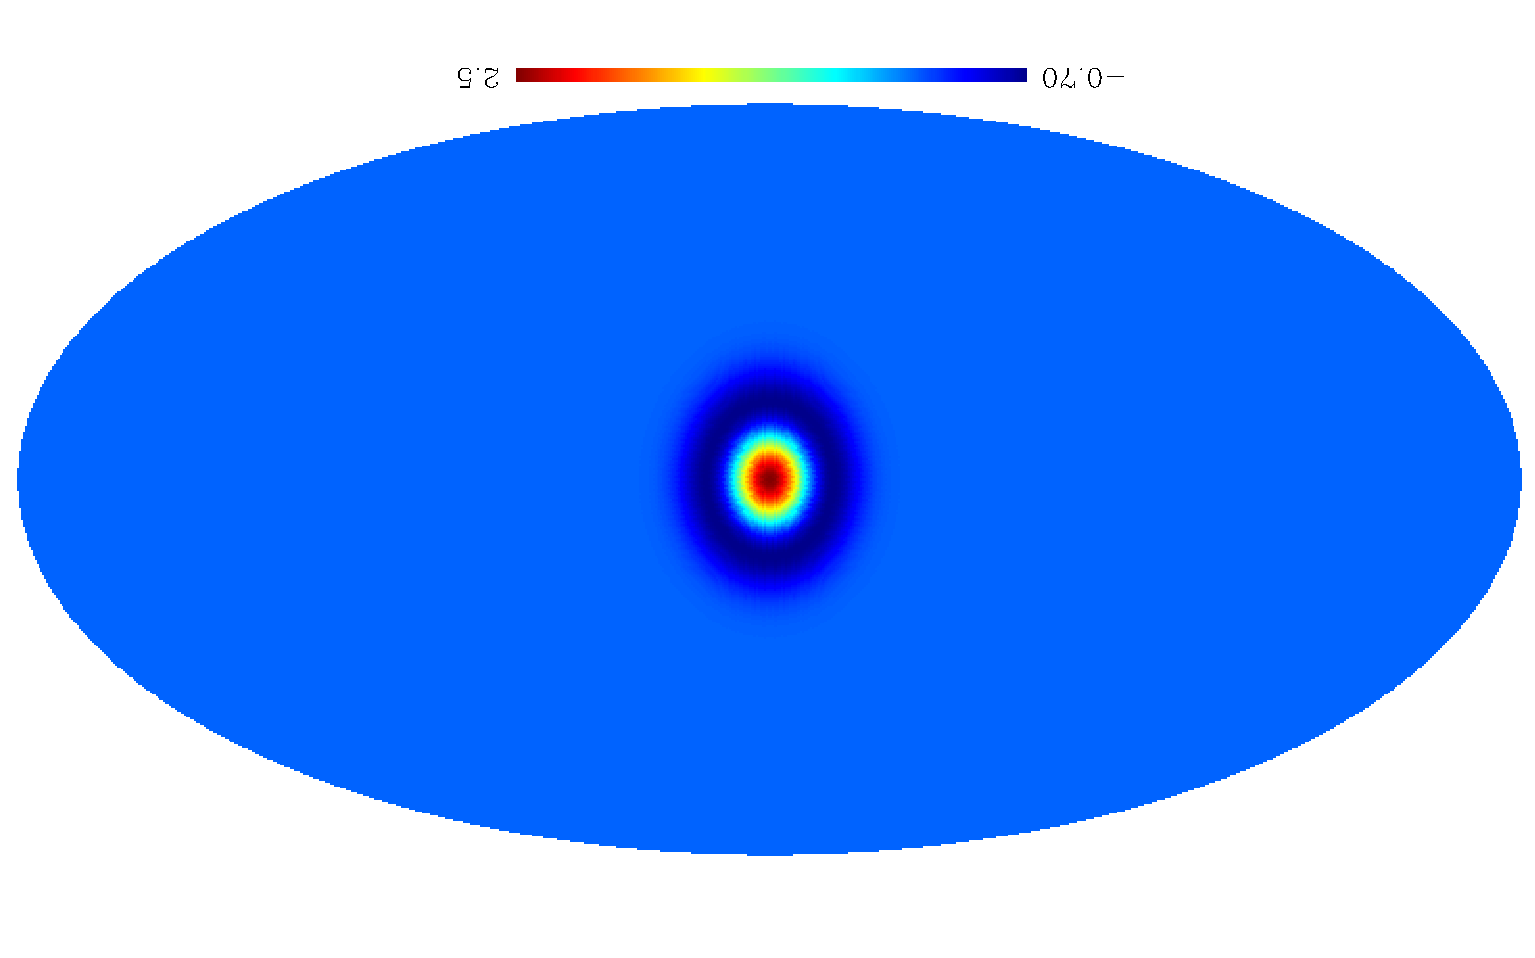
\includegraphics[angle=180,width=7.9cm]{wav_mex_hat_3.pdf}
}}
}
\caption{Mexican hat on the sphere for the dilation parameter equal to $a = \{1,2,4,8\}$.}
\label{fig_wav_mex_hat}
\end{figure}

% \begin{figure}[htb]
% \vbox{
% \centerline{
% \hbox{
% \includegraphics[angle=180,width=6.5cm]{mex_hat_0.pdf}
% \includegraphics[angle=180,width=6.5cm]{mex_hat_1.pdf}
% }}\centerline{
% \hbox{
% \includegraphics[angle=180,width=6.5cm]{mex_hat_8.pdf}
% \includegraphics[angle=180,width=6.5cm]{mex_hat_20.pdf}
% }}
% }
% \caption{Cosmic Microwave Background (CMB) simulated map and its mexican hat wavelet transform
% with dilation parameter $a = \{1,8,20\}$.}
% \label{fig_trans_cmb_wav_mex_hat}
% \end{figure}

The 2D Mexican hat wavelet transform is the second derivative of a Gaussian:
\begin{equation}
\label{rad_mexhat}
\psi(r) = \frac{1}{\sqrt{2 \pi}} \frac{1}{a} \Big( 2 - \Big( \frac{r}{a} \Big)^2 \Big) e^{- \frac{r^2}{2a^2}}
\end{equation}
where  $a$ is a scale factor parameter and $r$ the distance to the wavelet center.

Using the inverse stereographic projection, it is possible to extend the Mexican hat wavelet
on the sphere  \citep{wave:antoine99,wave:tenerio99,wave:cayon01,wave:holschneider96,wave:vielva04}:
\begin{equation}
\psi_a (r) = \frac{1}{\sqrt{2 \pi} C_a} \Big( 1 +  \Big( \frac{r}{2} \Big)^2 \Big)^2   \Big( 2 - \Big( \frac{r}{a} \Big)^2 \Big) e^{- \frac{r^2}{2a^2}}
\end{equation}
where $a$ is a scale factor, $C_a$ is a normalization term $C_a = a \Big( 1 + \frac{a^2}{2} + \frac{a^4}{4} \Big)^{\frac{1}{2}}$, 
and $r$ is the distance on the tangent plane, which is related to the polar angle $\theta$ through $r = 2 \textrm{tan} \frac{\theta}{2}$. 
This transform may be useful to analyze the data, but it does not have a reconstruction operator, and can therefore not be used for 
restoration applications.

Fig.~\ref{fig_wav_mex_hat} shows the Mexican hat wavelet on the sphere for four different scales.
%  and Fig ~\ref{fig_trans_cmb_wa_mex_hat}  shows four scales for the a simulated CMB map.


\subsection{Directional Wavelets}
\label{dirwavelet}
\index{wavelet!directional wavelets}

% \index{sphere!directionnal wavelet}

\begin{figure}[htb]
\centering
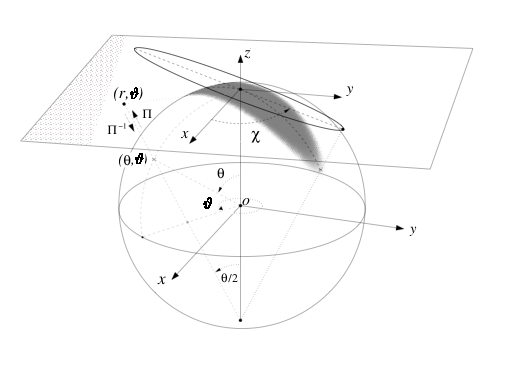
\includegraphics[width=15cm]{projection_stereo_ondelette_directionnelle.pdf}
\caption{Inverse stereographic projections  of a  directional wavelet on the sphere.}
\label{figprojstereo_direct2}
\end{figure}

To study anisotropic structures, the previously described continuous wavelet transform can be extended to directional wavelets \citep{wave:antoine01,vielva06,McEwen08}.
Fig.~\ref{figprojstereo_direct2} shows the projection of an elliptic function from the plane to the sphere.  

\subsubsection{Elongated Mexican Hat Wavelet}
\index{wavelet!mexican hat}

\begin{figure}[htb]
\vbox{
\centerline{
\hbox{
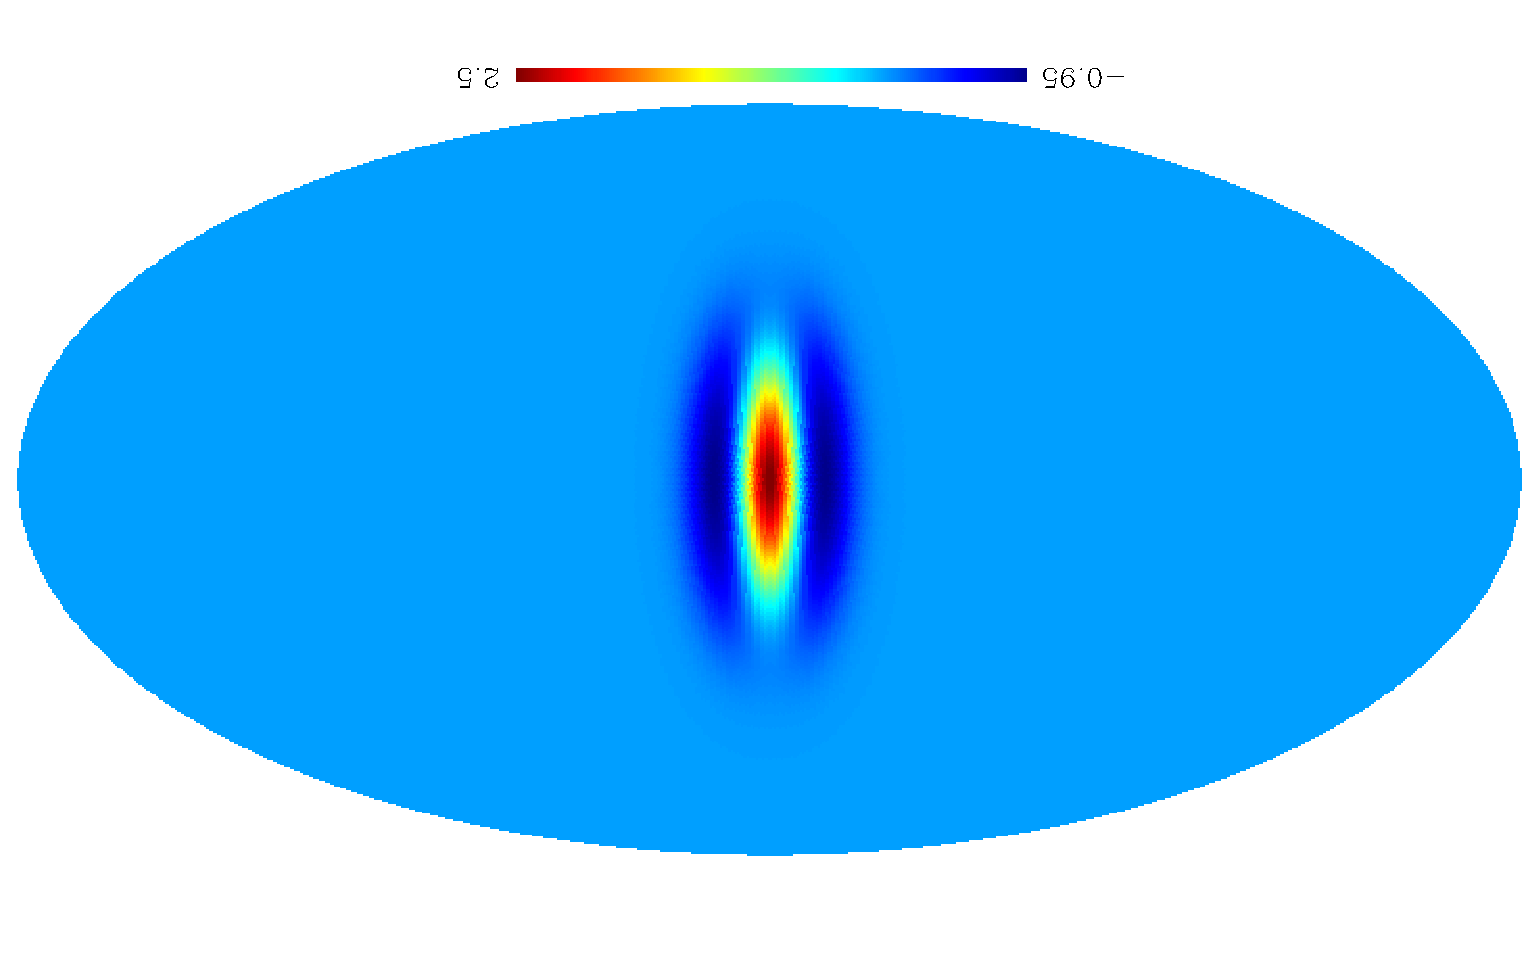
\includegraphics[angle=180,width=7.7cm]{dir_mex_hat_0.pdf}
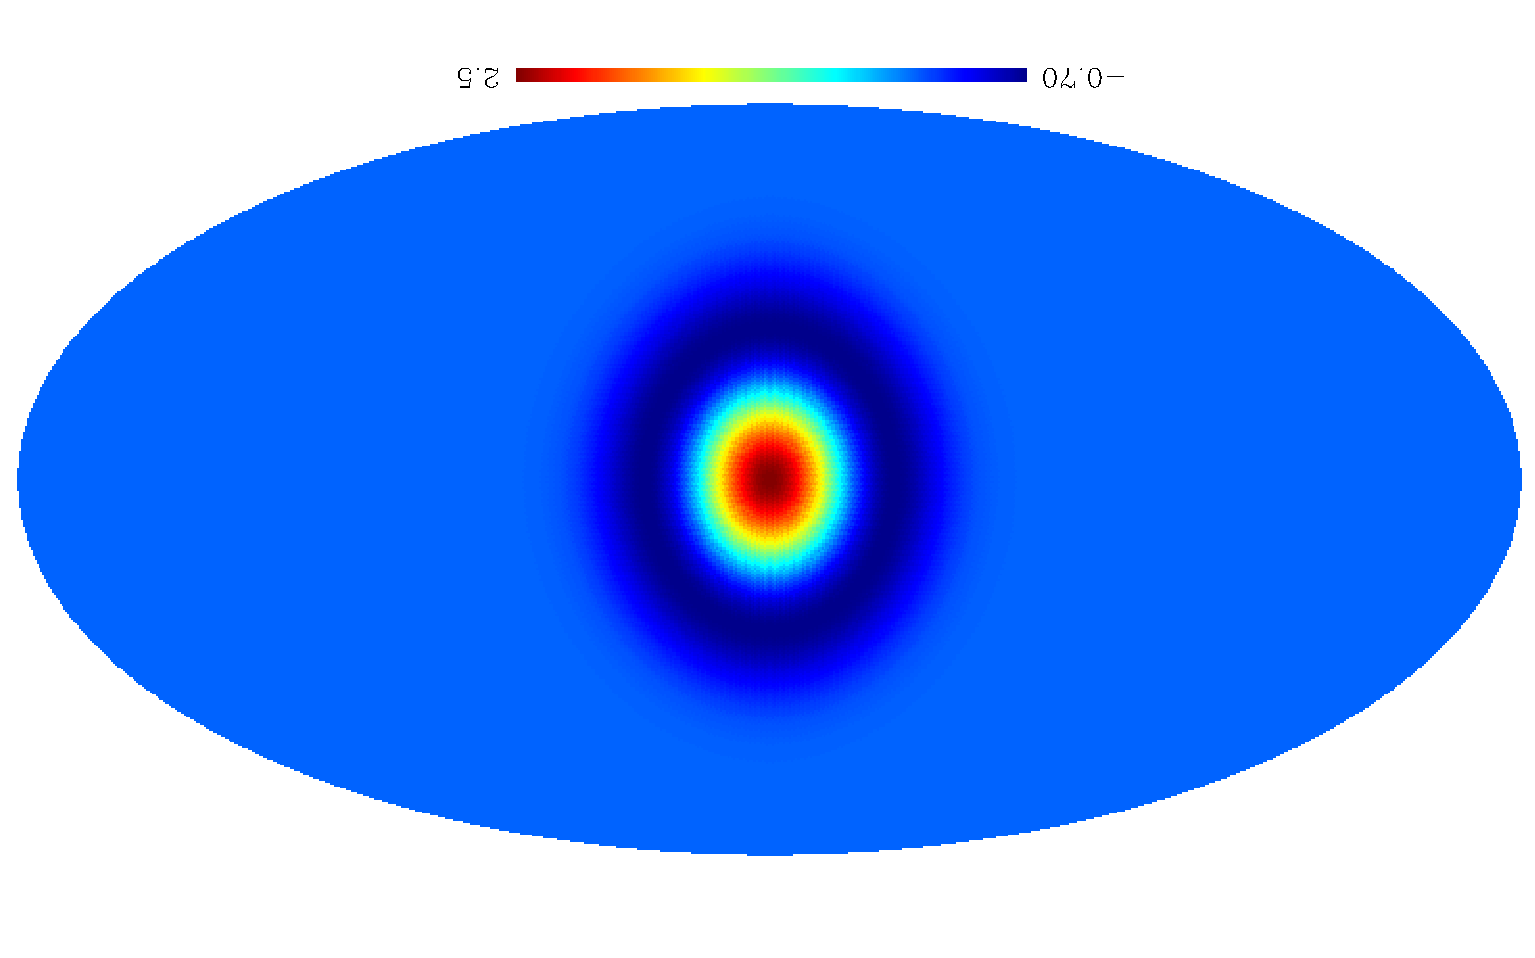
\includegraphics[angle=180,width=7.7cm]{dir_mex_hat_1.pdf}
}}\centerline{
\hbox{
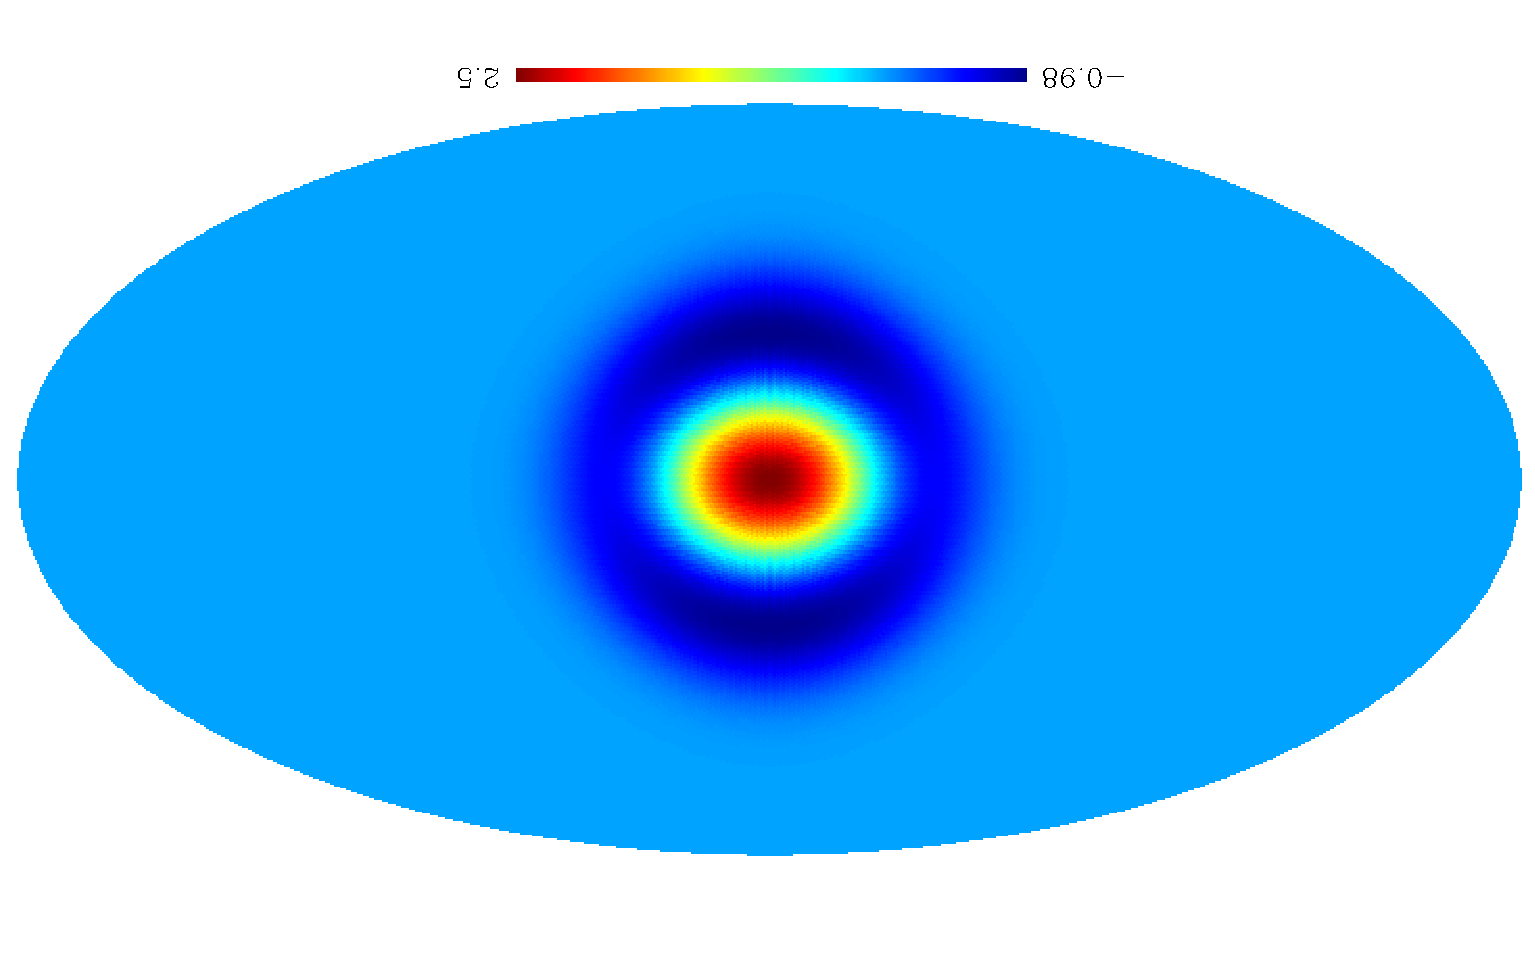
\includegraphics[angle=180,width=7.7cm]{dir_mex_hat_2.pdf}
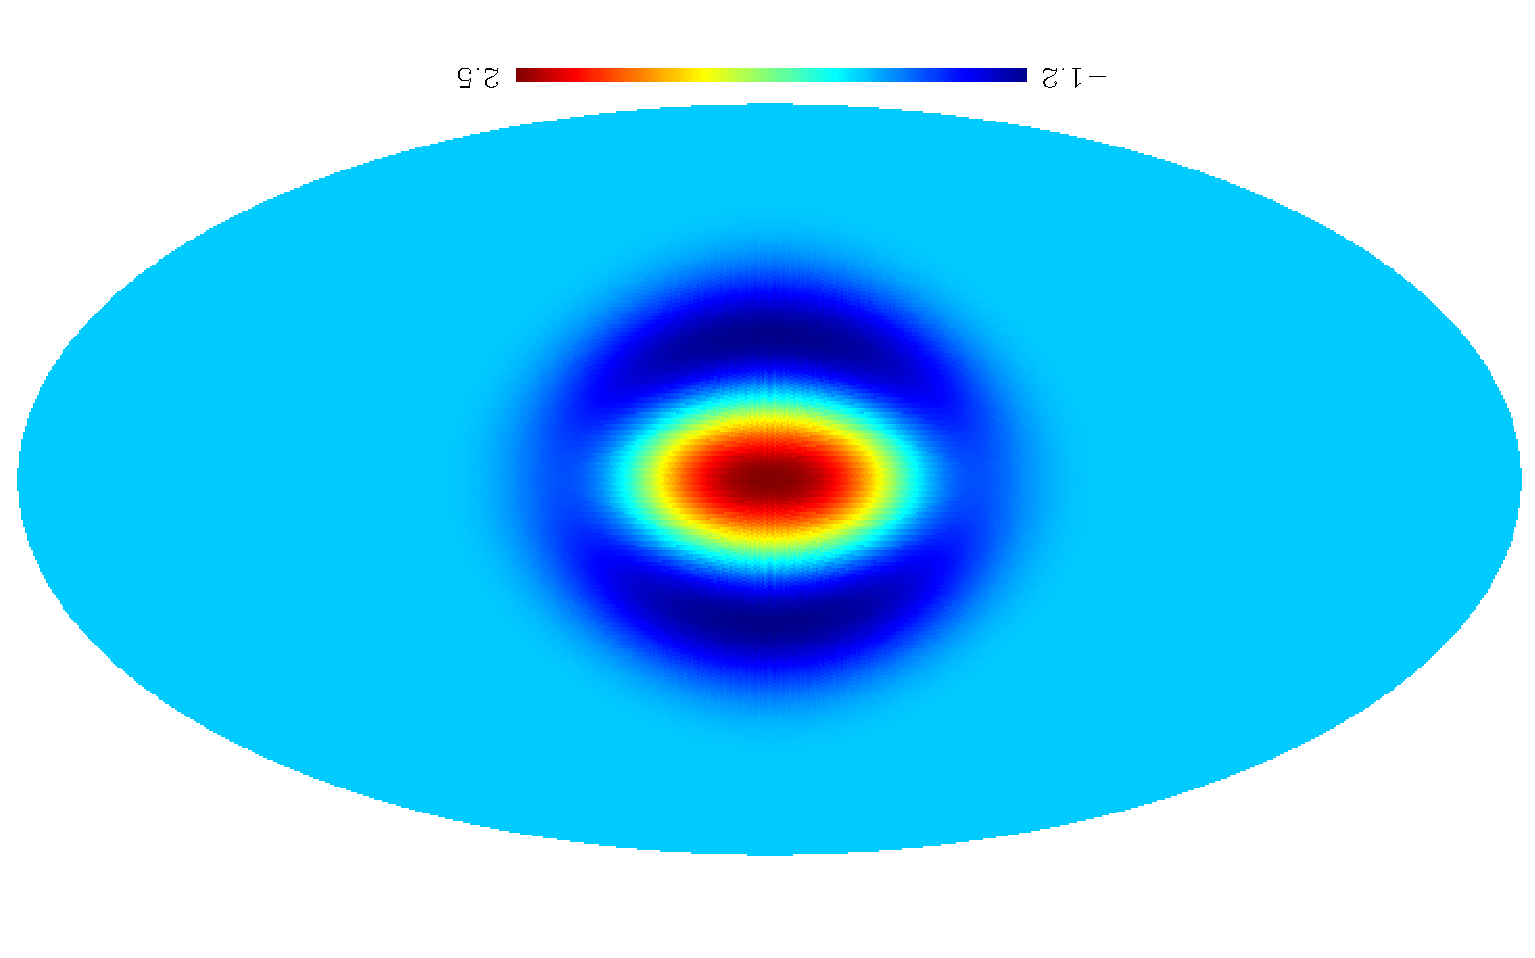
\includegraphics[angle=180,width=7.7cm]{dir_mex_hat_3.pdf}
}}
\centerline{
\hbox{
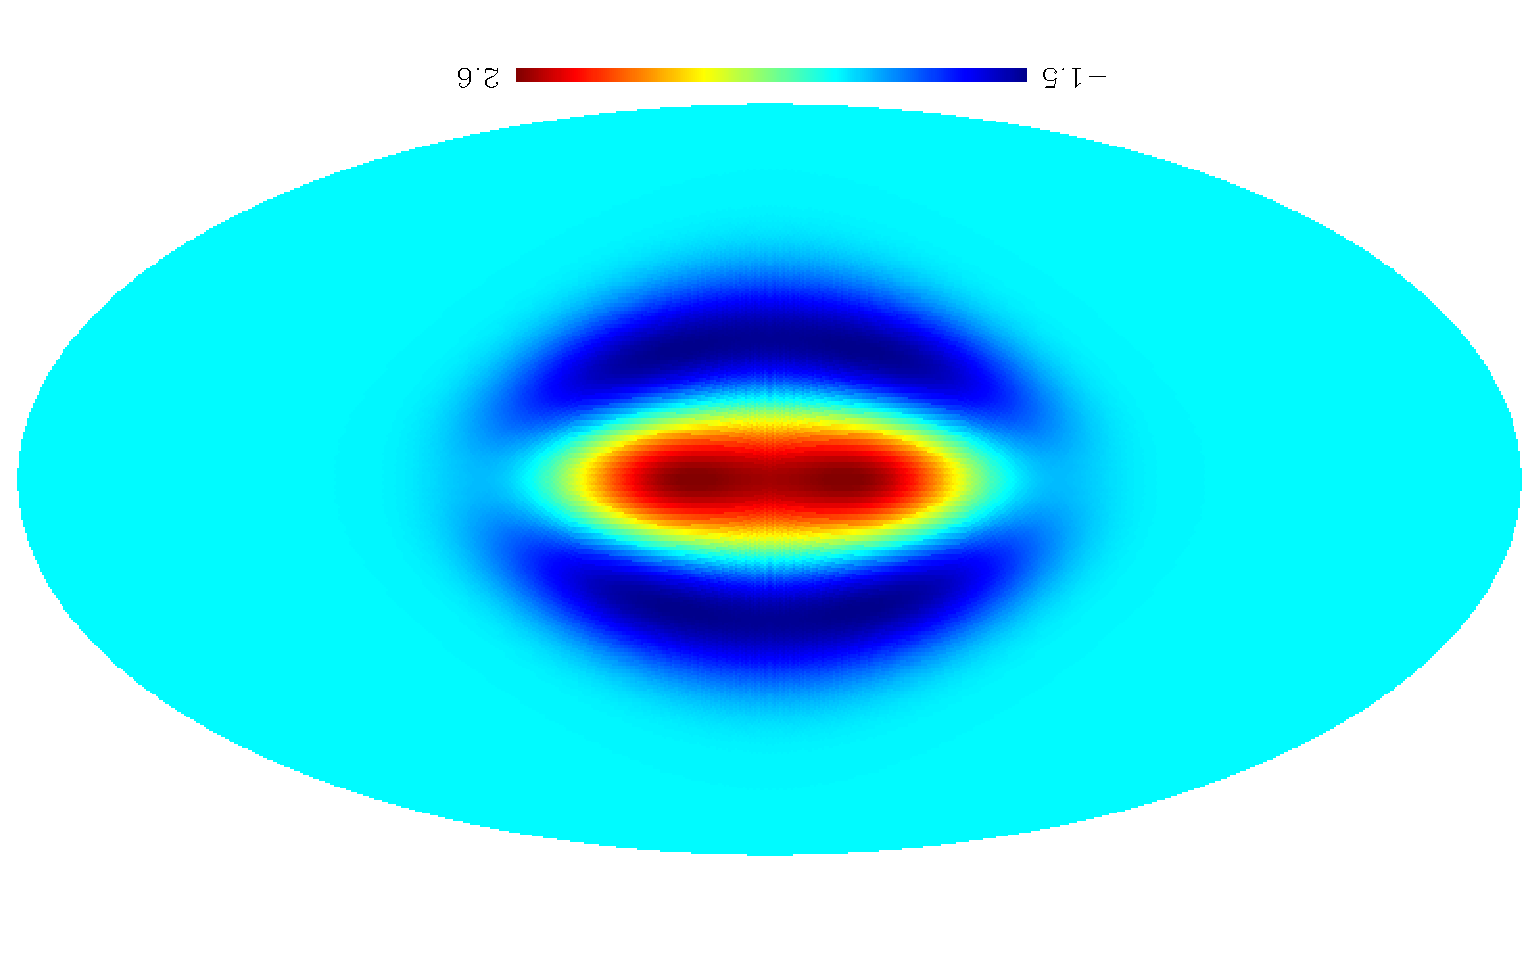
\includegraphics[angle=180,width=7.7cm]{dir_mex_hat_4.pdf}
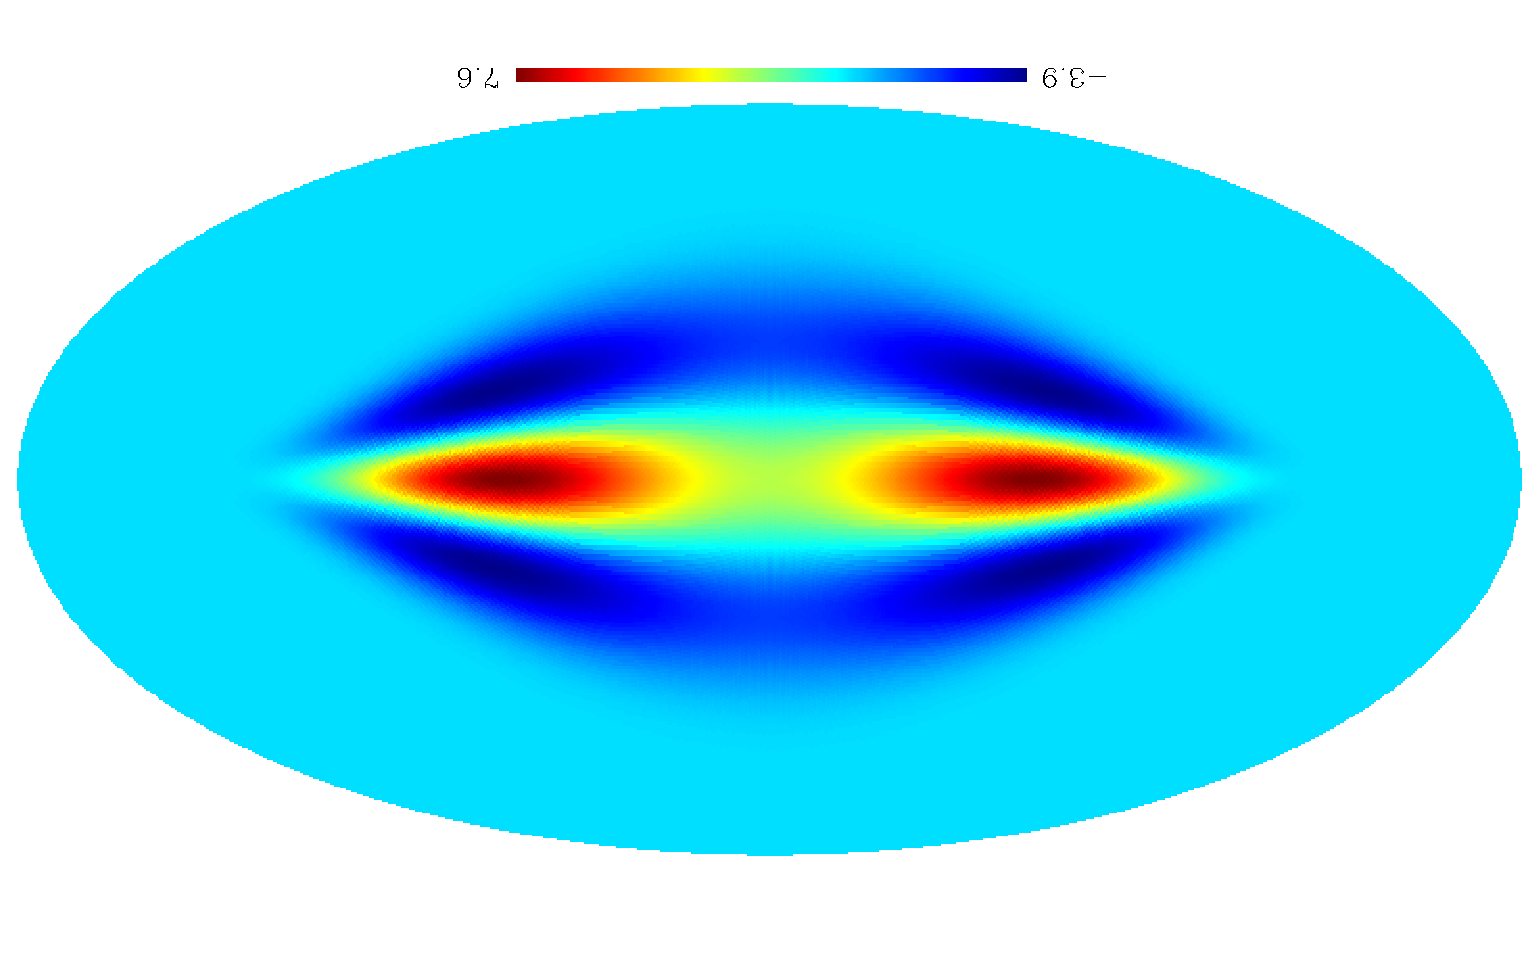
\includegraphics[angle=180,width=7.7cm]{dir_mex_hat_5.pdf}
}}
}
\caption{Elongated Mexican hat on the sphere for the dilation parameter equal to $a_x= 1$ and $a_y = \{0.5,1.,1.25,1.5,2,4\}$.}
\label{fig_dir_mex_hat}
\end{figure}

The elongated Mexican hat wavelet can be written as:
\begin{multline}
\label{directional_hat}
\psi_{a_x, a_y}(\theta, \vartheta) = \sqrt{\frac{2}{\pi}} C(a_x,a_y) \parenth{1+ \tan^2 \frac{\theta}{2}} \bigg( 1- \frac{4 \tan^2 \theta/2 }{a_x^2+a_y^2} \Big(\frac{a_y^2}{a_x^2} \cos^2 \vartheta \\
+  \frac{a_x^2}{a_y^2} \sin^2 \vartheta\Big) \bigg)  e^{-2 \tan \frac{\theta}{2}(\cos^2 \vartheta / a^2_x + \sin^2 \vartheta / a^2_y  )} ~
\end{multline}
where $a_x$ and $a_y$ are the dilation factors along the two axes $O_x$ and $O_y$, $C(a_x,a_y)$ is a normalization constant defined as
\begin{eqnarray}
\label{directional_hat_norm}
C(a_x,a_y)& =& (a_x^2+a_y^2) \parenth{a_x a_y (3a_x^4+ 3a_y^4+2a_xa_y)}^{-1/2} ~
\end{eqnarray}

Fig.~\ref{fig_dir_mex_hat} shows the wavelet functions for different dilation parameters $a_x$ and $a_y$.


\subsubsection{Morlet Wavelet}
\index{wavelet!Morlet}

\begin{figure}[htb]
\vbox{
\centerline{
\hbox{
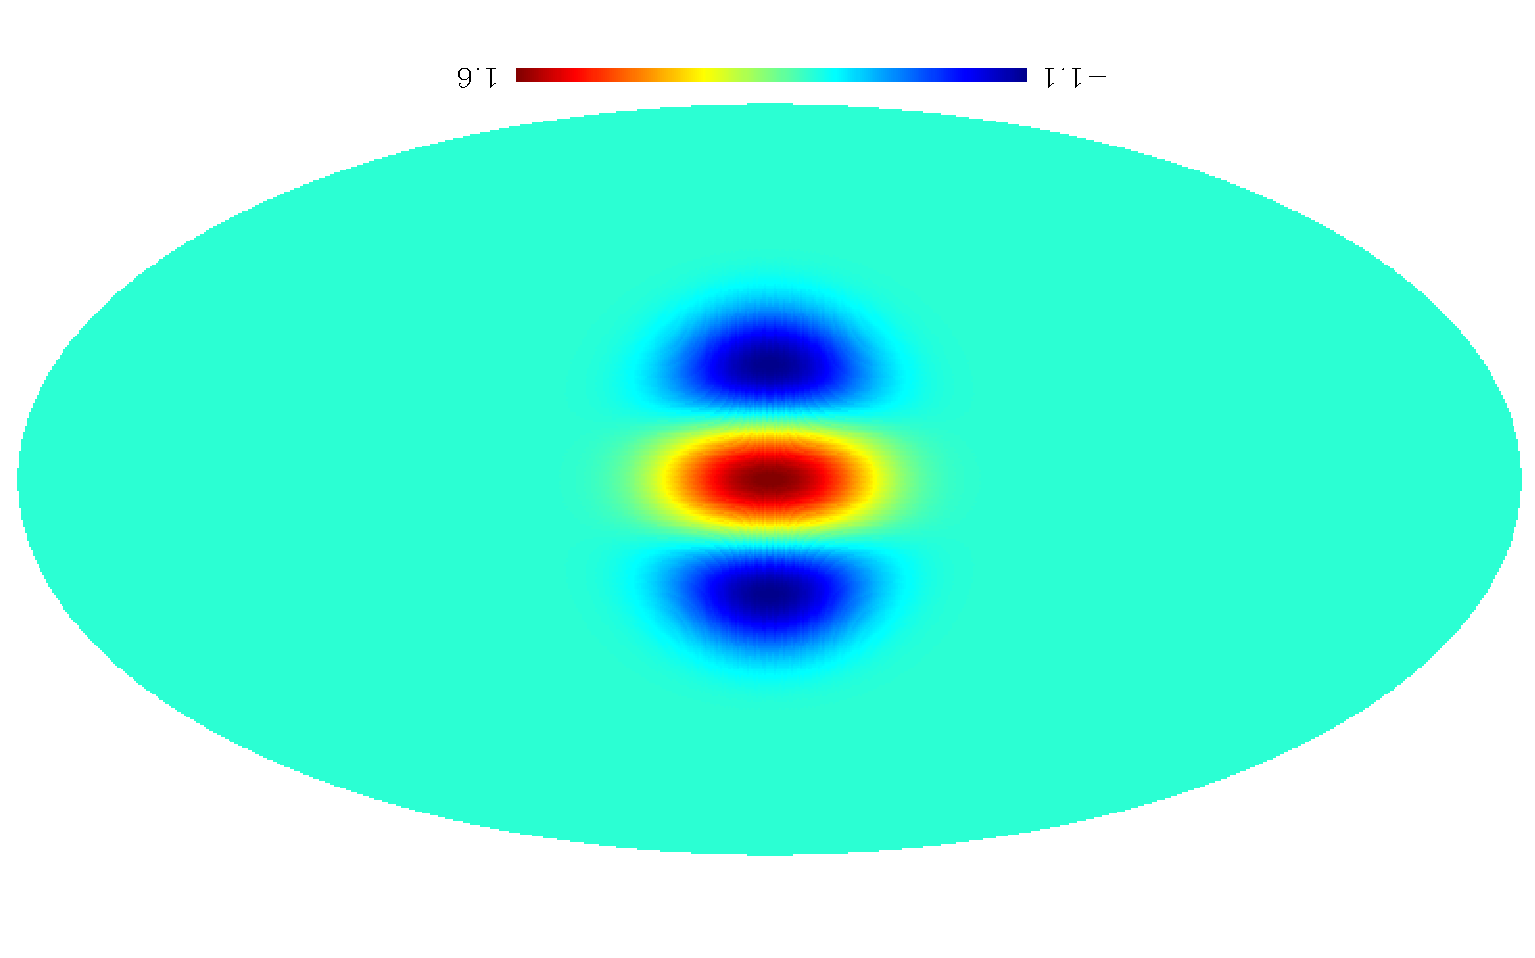
\includegraphics[angle=180,width=7.9cm]{dir_morlet_0.pdf}
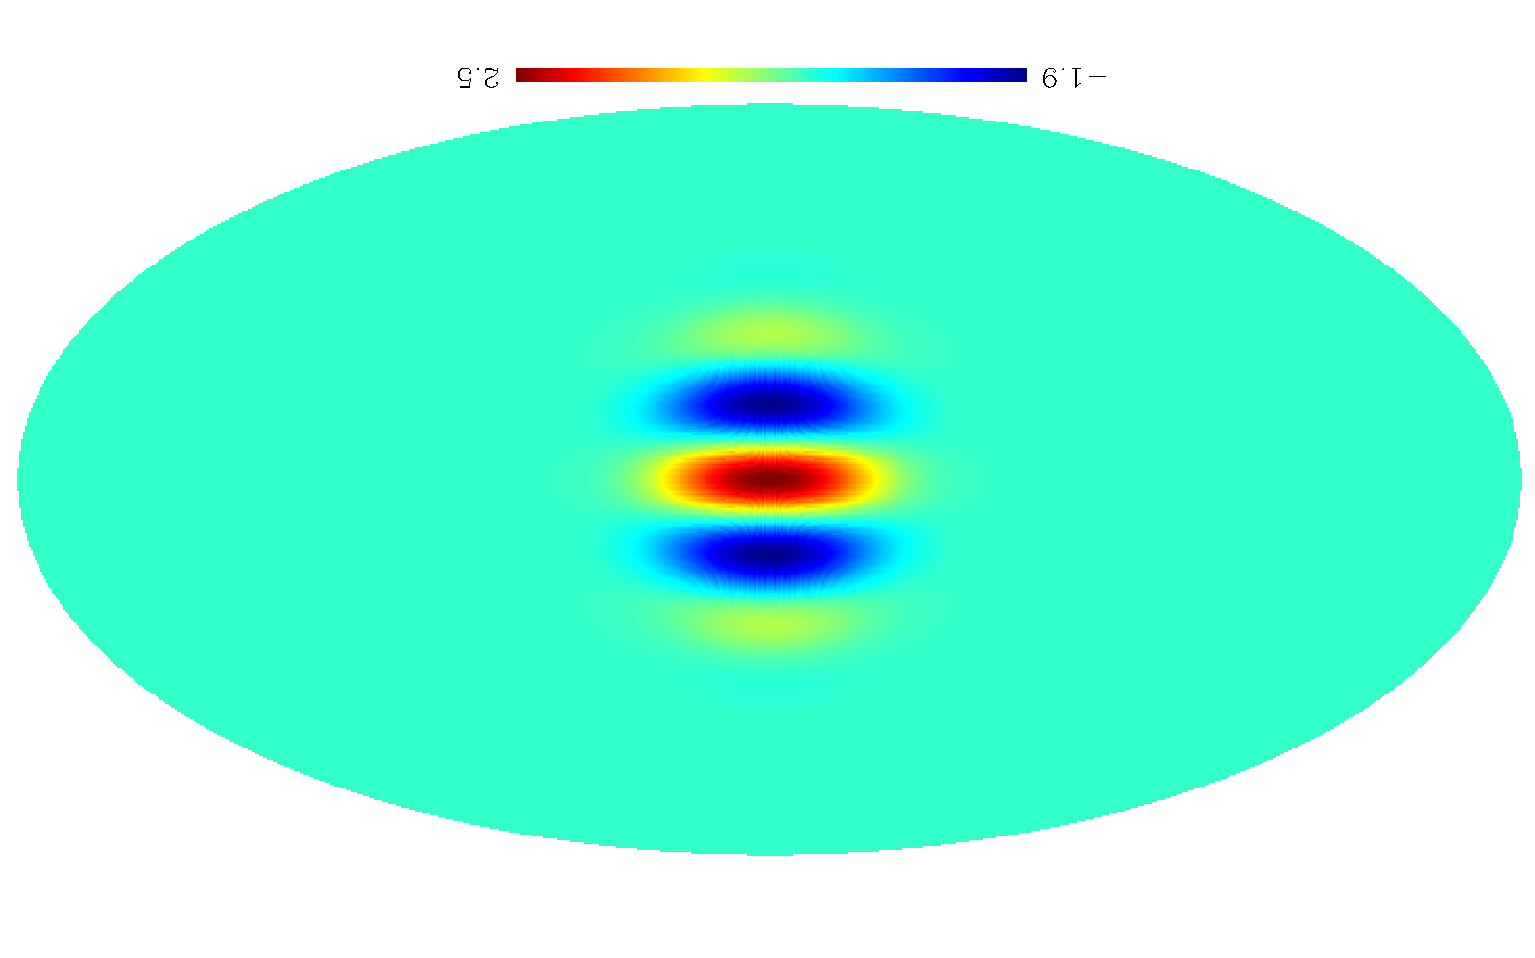
\includegraphics[angle=180,width=7.9cm]{dir_morlet_1.pdf}
}}\centerline{
\hbox{
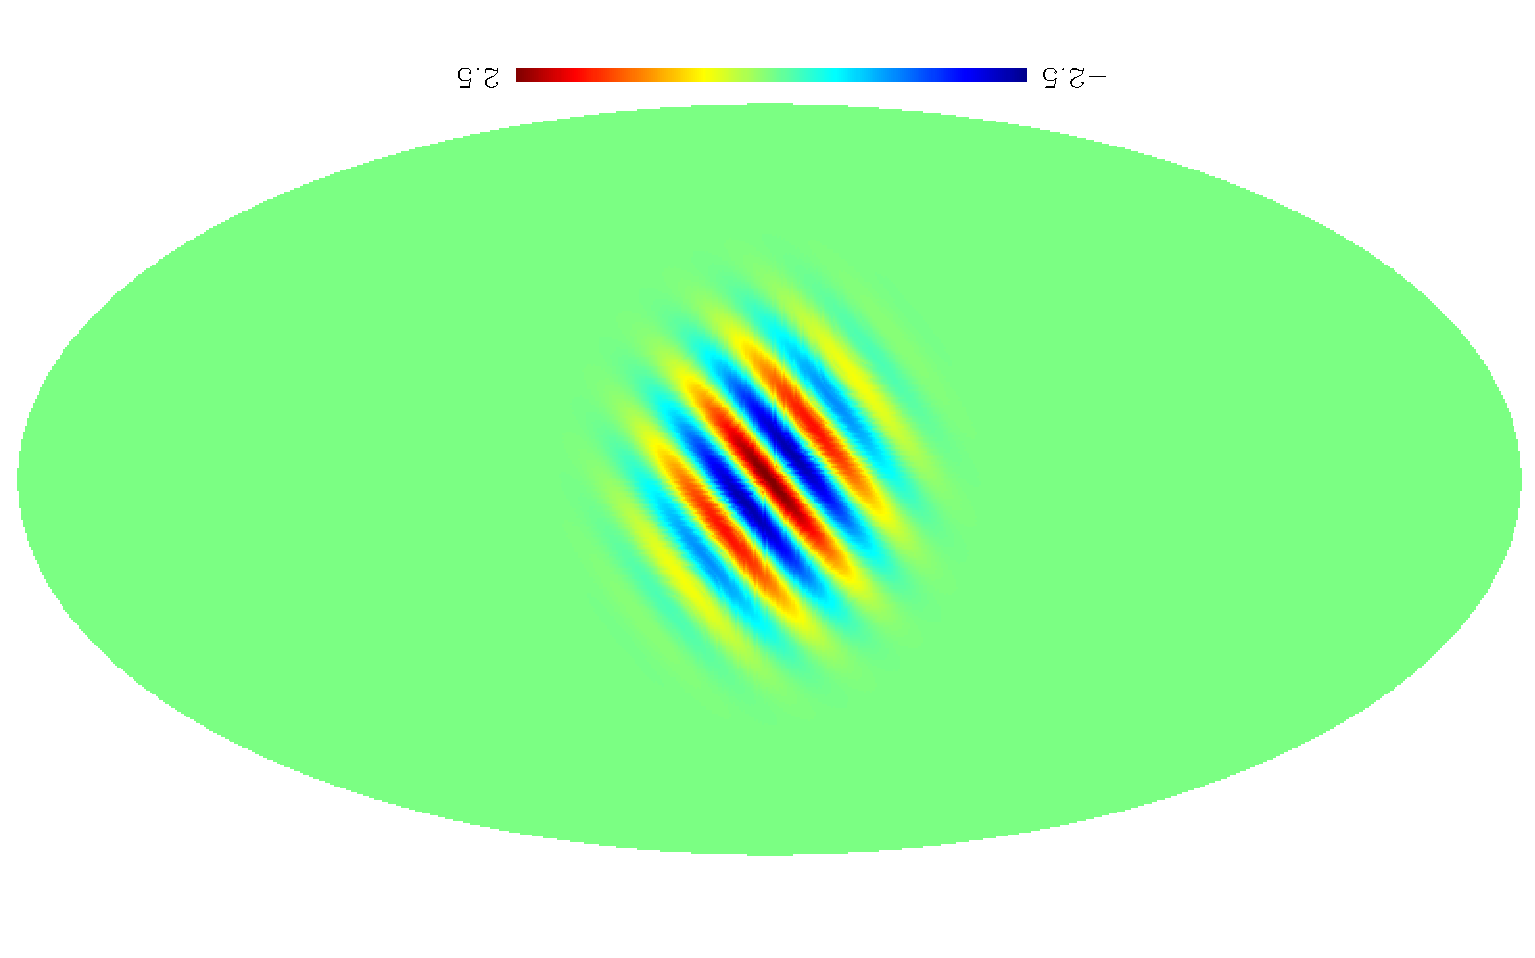
\includegraphics[angle=180,width=7.9cm]{dir_morlet_2.pdf}
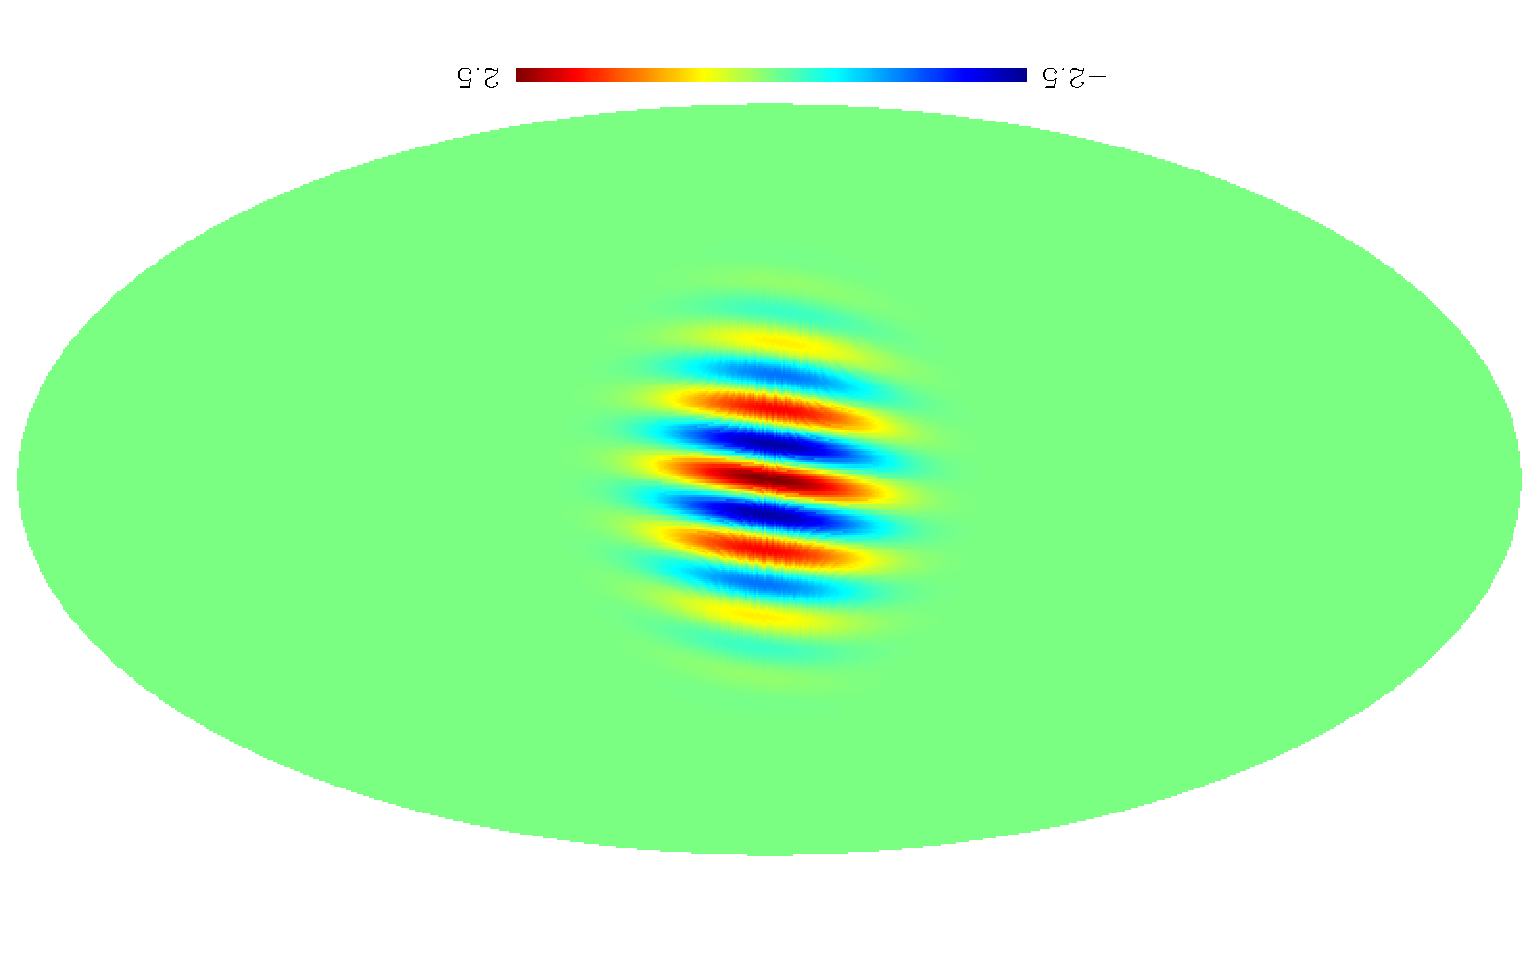
\includegraphics[angle=180,width=7.9cm]{dir_morlet_3.pdf}
}}
}
\caption{Morlet wavelets on the sphere for the parameter  $\bk$ equal to  (2,0), (4,0), (6,6) et (9,1).}
\label{fig_dir_morlet}
\end{figure}

The Morlet wavelet on the sphere, derived from the stereographic projection of the 2D function on the plane, is:
\begin{equation}
\label{real_morlet}
\psi_{a_x, a_y, {\bf k}}(\theta, \vartheta) = \sqrt{\frac{2}{\pi}} C({\bf k}) (1+ \tan^2 \frac{\theta}{2}) \bigg(\cos \frac{ {\bf k} \cdotp R^{-1} {\bf x} }{\sqrt{2}} - e^{- |{\bf k}|^2/4} \bigg) e^{-2 \tan^2(\theta/2)} 
\end{equation}
with $R^{-1} {\bf x} = (2 \tan (\theta/2) \cos \vartheta,2 \tan (\theta/2) \sin \vartheta)$, ${\bf k}=(k_x,k_y)$, $|{\bf k}|^2 = k_x^2 + k_y^2$, 
and $C({\bf k}) = (1+3e^{-|{\bf k}|^2/2} -4e^{-3 |{\bf k}|^2/8})^{-1/2} $. ${\bf k}$ allows us to control the oscillations of the wavelet functions.\\ \\
Fig.~\ref{fig_dir_morlet} shows the Morlet wavelet for ${\bf k}$ equal respectively to $(2,0)$, $(4,0)$, $(6,6)$ and $(9,1)$.\\

Continuous wavelet transforms have been intensively used in astrophysics, mainly to analyze the Cosmic Microwave Background \citep{wave:vielva04}.
Directional wavelets based on steerable filters were also proposed in \citep{wiaux06,McEwen08}. We present in the following a set of multiscale 
decompositions on the sphere which have a fast exact inverse transform, and are therefore suitable for many applications such as restoration.
 



%===============================================================

\section{Redundant Wavelet Transform on the Sphere with Exact Reconstruction}
\label{sect_wts}
%We show in this section that we can build  wavelet transforms on the sphere, based on the spherical harmonics transform, ewhich have an exact reconstruction and can therefore be easily used in different applications.


\subsection{Isotropic Undecimated Wavelet Transform on the Sphere}
Here an undecimated isotropic transform (UWTS) is described which is similar in many respects to the undecimated isotropic transform 
\citep{starck2010,starck:sta06}, and will therefore be a good candidate for restoration applications. Its isotropy is a favorable 
property when analyzing isotropic features. This isotropic transform is obtained using a scaling function ${\phi}_{l_c}(\theta, \vartheta)$ 
with cut-off frequency  $l_c$ and  azimuthal symmetry, meaning that ${\phi}_{l_c}$ does not depend on the azimuth $\vartheta$. 
Hence the spherical harmonics coefficients $\hat {\phi}_{l_c} [l,m]$ of ${\phi}_{l_c}$ vanish when $m \ne 0$ so that:
\begin{eqnarray}
{\phi}_{l_c}(\theta, \vartheta)= {\phi}_{l_c}(\theta) = \sum_{l = 0}^{l = l_c} \hat  {\phi}_{l_c} [l,0] Y_{l0}(\theta, \vartheta) .
\end{eqnarray}
Then, convolving a function $f(\theta, \vartheta) \in L_2(S^2)$ with ${\phi}_{l_c}$ is greatly simplified 
and the spherical harmonics coefficients of the resulting map $c_0$ are readily given by
\begin{eqnarray}
 \hat c_{0}[l,m] = \widehat{{\phi}_{l_c} * f} [l,m] = \sqrt{\frac{2l+1}{4\pi} } \hat {\phi}_{l_c} [l,0] \hat f[l,m]  .
\end{eqnarray}
\index{sphere!undecimated wavelet}

\subsubsection{From One Resolution to the Next}

A sequence of smoother approximations of $f$ on a dyadic resolution scale can be obtained using the scaling function ${\phi}_{l_c}$ as follows:
\begin{eqnarray}
\begin{split}
c_0   & = &  {\phi}_{ l_{c} }  \ast f        \\
c_1   & = &  {\phi}_{2^{-1} l_{c} }   \ast f    	   \\
&\ldots&\\ 
c_j    &=&   {\phi}_{2^{-j}  l_{c}  }  \ast f  ,
\end{split}
\end{eqnarray}
where ${\phi}_{2^{-j} l_{c} }$ is a rescaled version of ${\phi}_{l_{c}}$. The above multiresolution sequence can actually  be obtained recursively. 

Define a low pass filter $h_{j}$ for each scale $j$  by:
\begin{eqnarray}
 \widehat{H}_{j}[l,m]  & = & \sqrt{\frac{4\pi}{2l+1} }  \hat h_{j}[l,m]   \nonumber  \\
   &  = & 
   \begin{cases}
   \frac {   \hat \phi_{\frac{l_{c}}{2^{j+1}} }[l,m]   }   {  \hat  \phi_{  \frac{l_{c}}{2^{j}} }[l,m]   } & \mbox{if }  l  < \frac{ l_{c}} {2^{j+1}} \quad \textrm{and}\quad m = 0 , \\
   0 & \mbox{otherwise } . 
  \end{cases}
\end{eqnarray}
It is then easily shown that $c_{j+1}$ derives from $c_j$ by convolution on the sphere with $h_j$:  $c_{j+1} = c_{j} \ast h_j$.


\subsubsection{The Wavelet Coefficients}

Given an axisymmetric  wavelet function $\psi_{l_c}$, we can derive in the same way a 
high pass filter $g_j$ on each scale~$j$:
\begin{eqnarray}
 \widehat{G}_{j}[l,m]  & = & \sqrt{\frac{4\pi}{2l+1} }  \hat{g}_{j}[l,m] \nonumber  \\
   & = & 
  \begin{cases}
  \frac {   \hat \psi_{\frac{l_{c}}{2^{j+1}} }[l,m]   }   {  \hat  \phi_{  \frac{l_{c}}{2^{j}} }[l,m]   } & \mbox{if }  l  < \frac{ l_{c}} {2^{j+1}} \quad \textrm{and}\quad m = 0 ,\\
1 &\mbox{if }  l  \ge \frac{ l_{c}} {2^{j+1}} \quad \textrm{and}\quad m = 0 ,\\ 
0&  \mbox{otherwise } .
  \end{cases}
\end{eqnarray}
From this definition, the wavelet coefficients $w_{j+1} $ at scale $j+1$ are obtained from the previous scaling coefficients $c_j$ 
by a simple convolution on the sphere with $g_j$: $w_{j+1} = c_{j} \ast g_j$.

As in the standard 2D isotropic undecimated transform algorithm, the wavelet coefficients can be defined as the difference between two consecutive resolutions, 
$w_{j+1}(\theta, \vartheta) = c_{j}(\theta, \vartheta) - c_{j+1}(\theta, \vartheta)$. This defines a zonal wavelet function $\psi_{l_c}$ as:
\begin{eqnarray}\label{wavelet}
\hat \psi_{\frac{l_c}{2^{j}}}[l,m] = \hat \phi_{\frac{l_c}{2^{j-1}}} [l,m]  - \hat \phi_{\frac{l_c}{2^{j}}}[l,m] .
\end{eqnarray}
The high pass filters $g_j$ associated with this wavelet are expressed as: 
\begin{eqnarray}
\begin{split}
\widehat{G}_{j}[l,m]  & = \sqrt{\frac{4\pi}{2l+1} } \hat{g}_{j}[l,m]  \\
                  & = 1 - \sqrt{\frac{4\pi}{2l+1} } \hat{h}_j[l,m]   =   1 - \widehat{H}_j[l,m] .
\end{split}
\end{eqnarray}
Obviously other wavelet functions could be used just as well. For example, we can define the wavelet function as the difference between
the squares of the scaling functions \cite{starck:book98}, i.e. $\hat \psi^2_{\frac{l_c}{2^{j}}}[l,m] = \hat \phi^2_{\frac{l_c}{2^{j-1}}} [l,m]  - \hat \phi^2_{\frac{l_c}{2^{j}}}[l,m]$. 

\newpage
\subsubsection{Choice of the Scaling Function}
\index{wavelet!needlet}
\index{wavelet!Meyer}

\begin{figure}[htb]
\vbox{
\centerline{
\hbox{
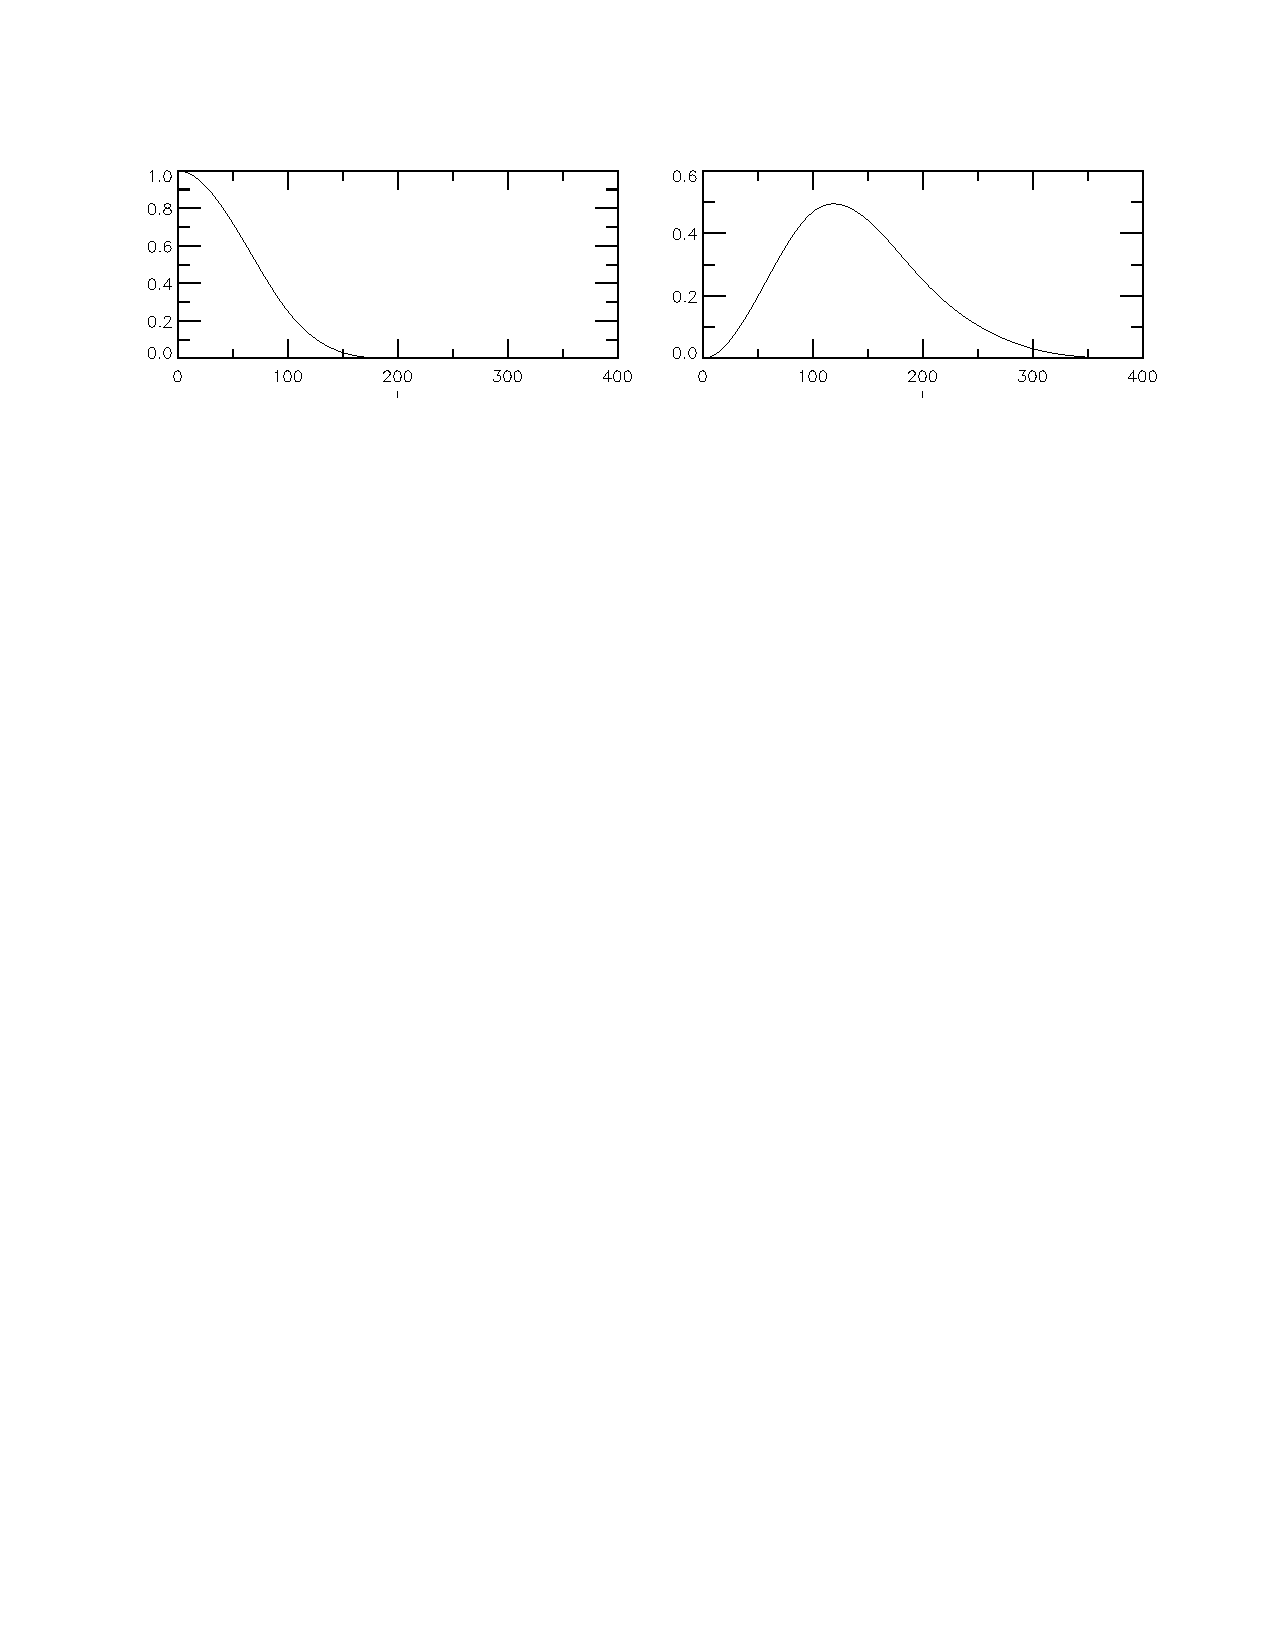
\includegraphics[width=15cm,height=5cm]{fig_sphere_filterbank1.pdf}
% 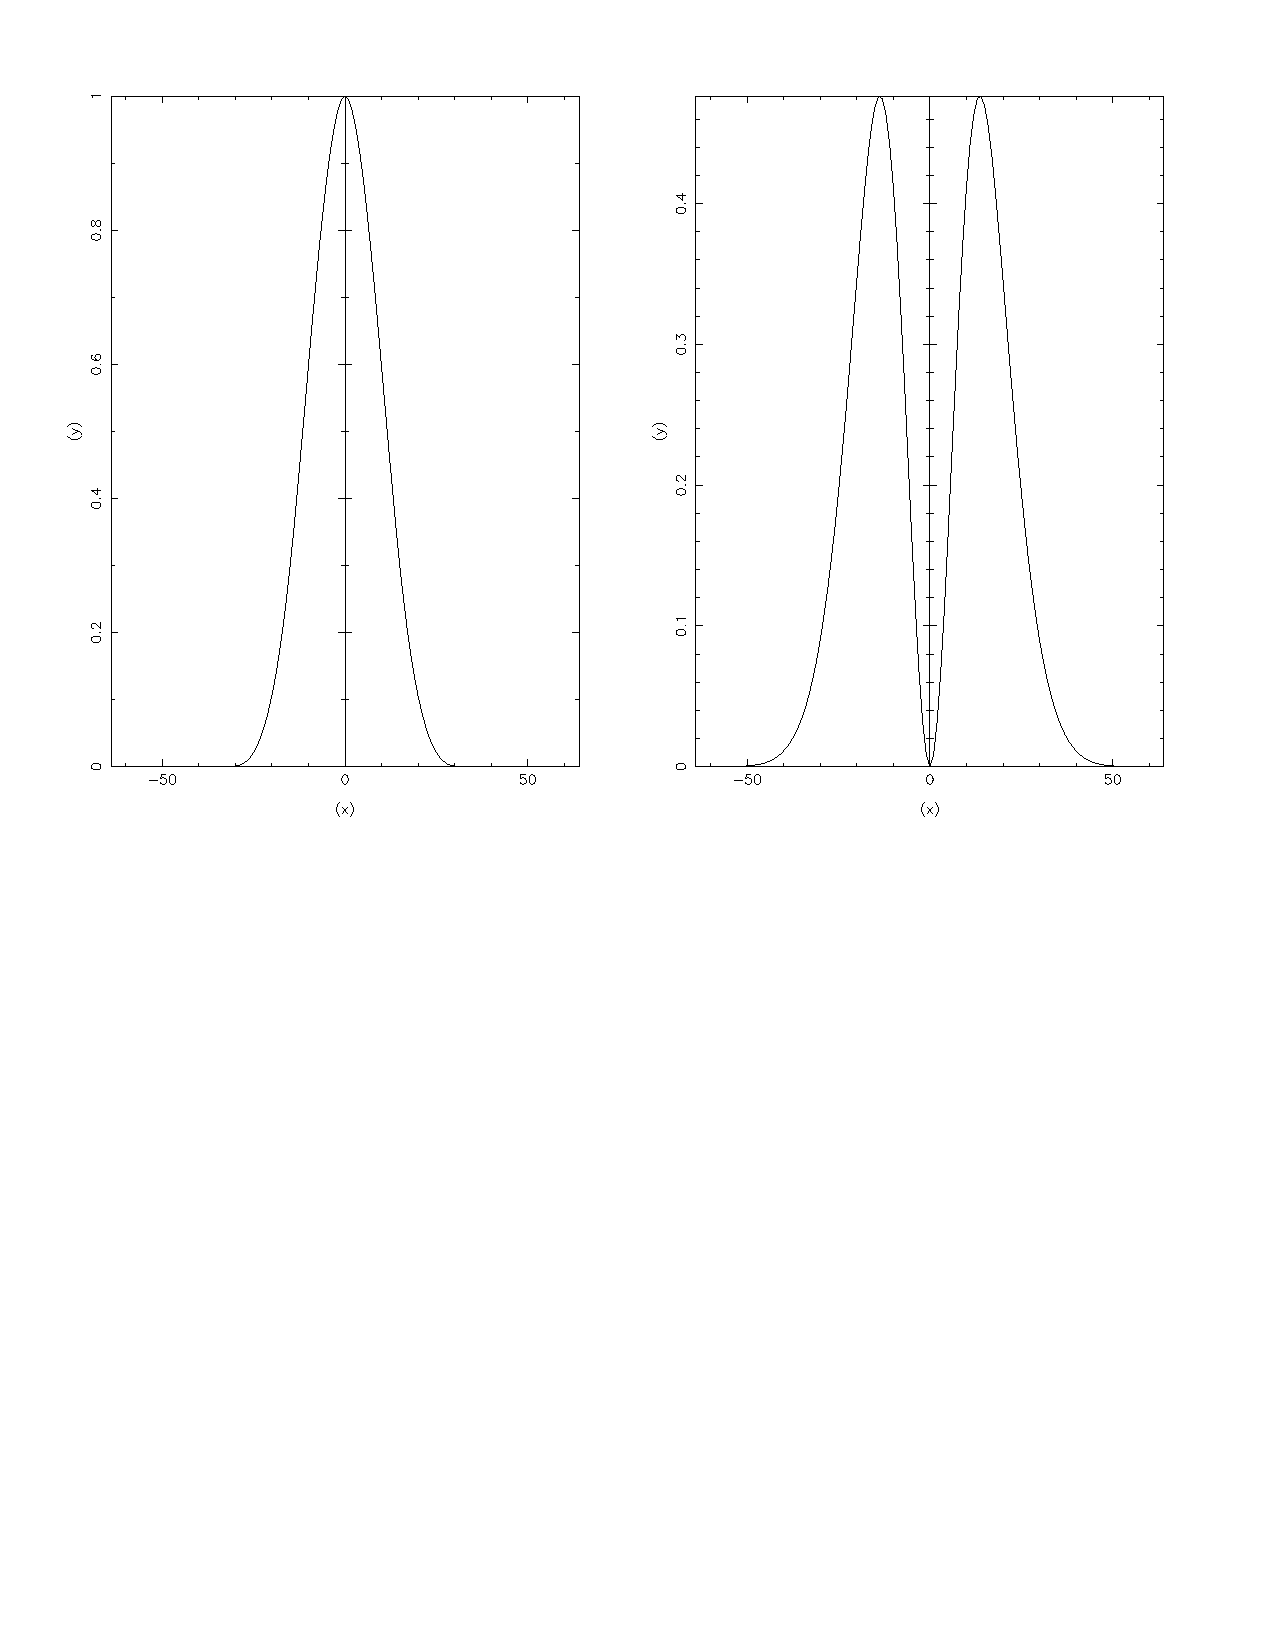
\includegraphics[width=14cm,height=5cm]{ch1_diff_uv_phi_psi.pdf}
}}}
\caption{On the left, spherical harmonics coefficients $\hat{{\phi}}[l,0]$ of the the scaling function ${{\phi}}$ and, on the right, those of the wavelet function ${\psi}$.}
\label{fig_diff_uv_phi_psi}
\end{figure}

\begin{figure}[htb]
\vbox{
\centerline{
\hbox{
 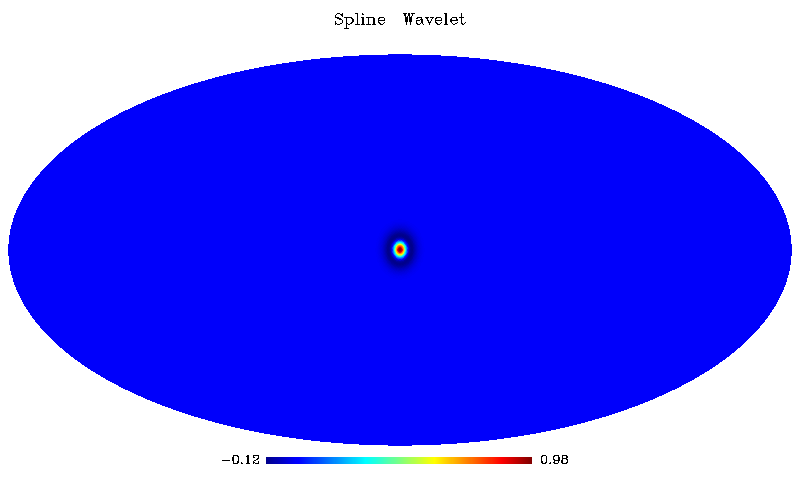
\includegraphics[width=7.5cm]{fig_splinew.png}%[width=6.5cm,height=3.9cm]
 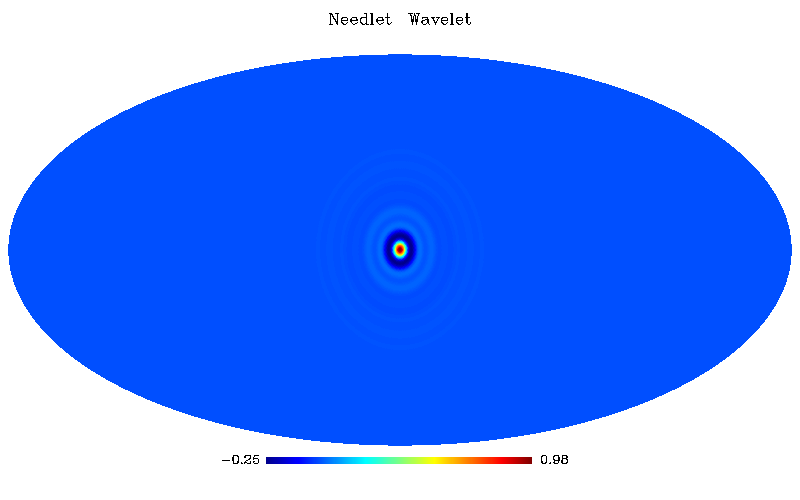
\includegraphics[width=7.5cm]{fig_needletw.png}
}}
\centerline{
\hbox{
 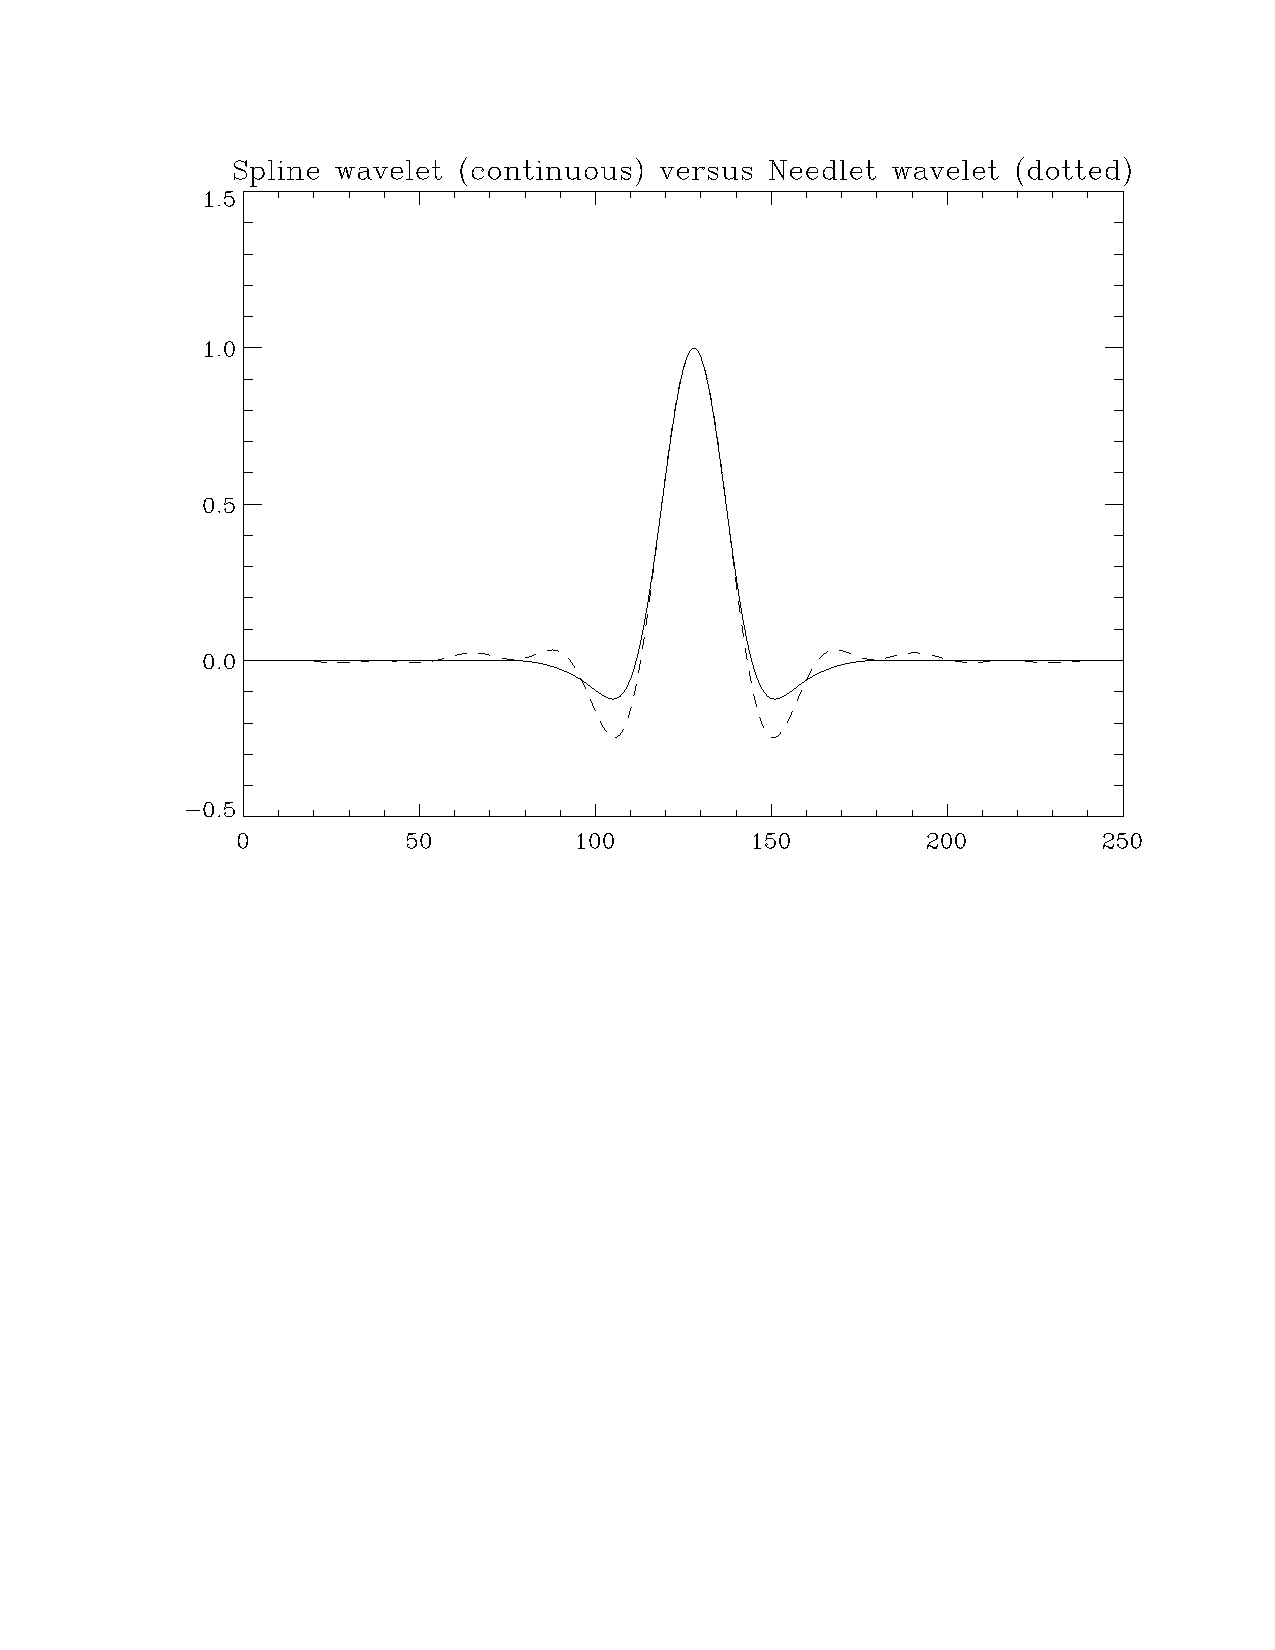
\includegraphics[width=7.5cm, trim= 2cm 14cm 2cm 2cm, clip=]{fig_splinew_versus_needletw.pdf}
 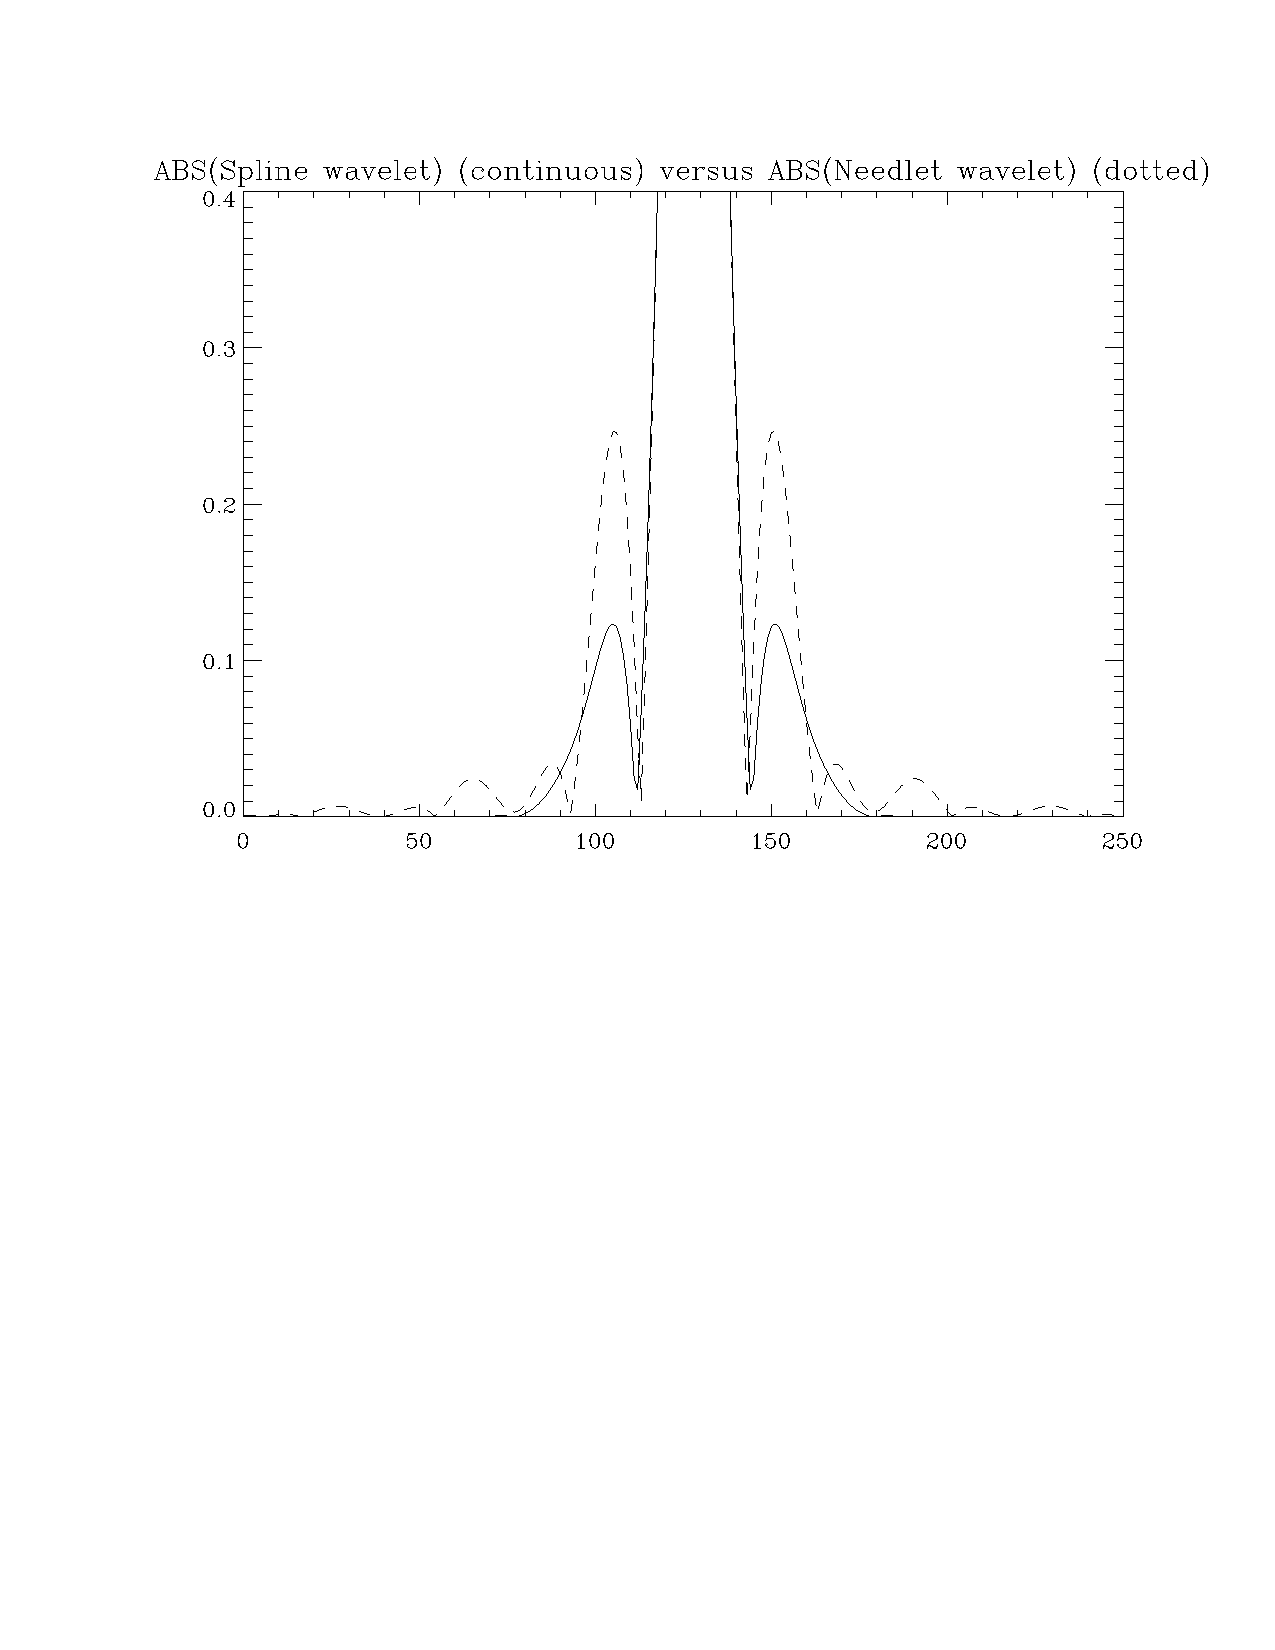
\includegraphics[width=7.5cm, trim= 2cm 14cm 2cm 2cm, clip=]{fig_abssplinew_versus_absneedletw.pdf}
}}
\centerline{
\hbox{
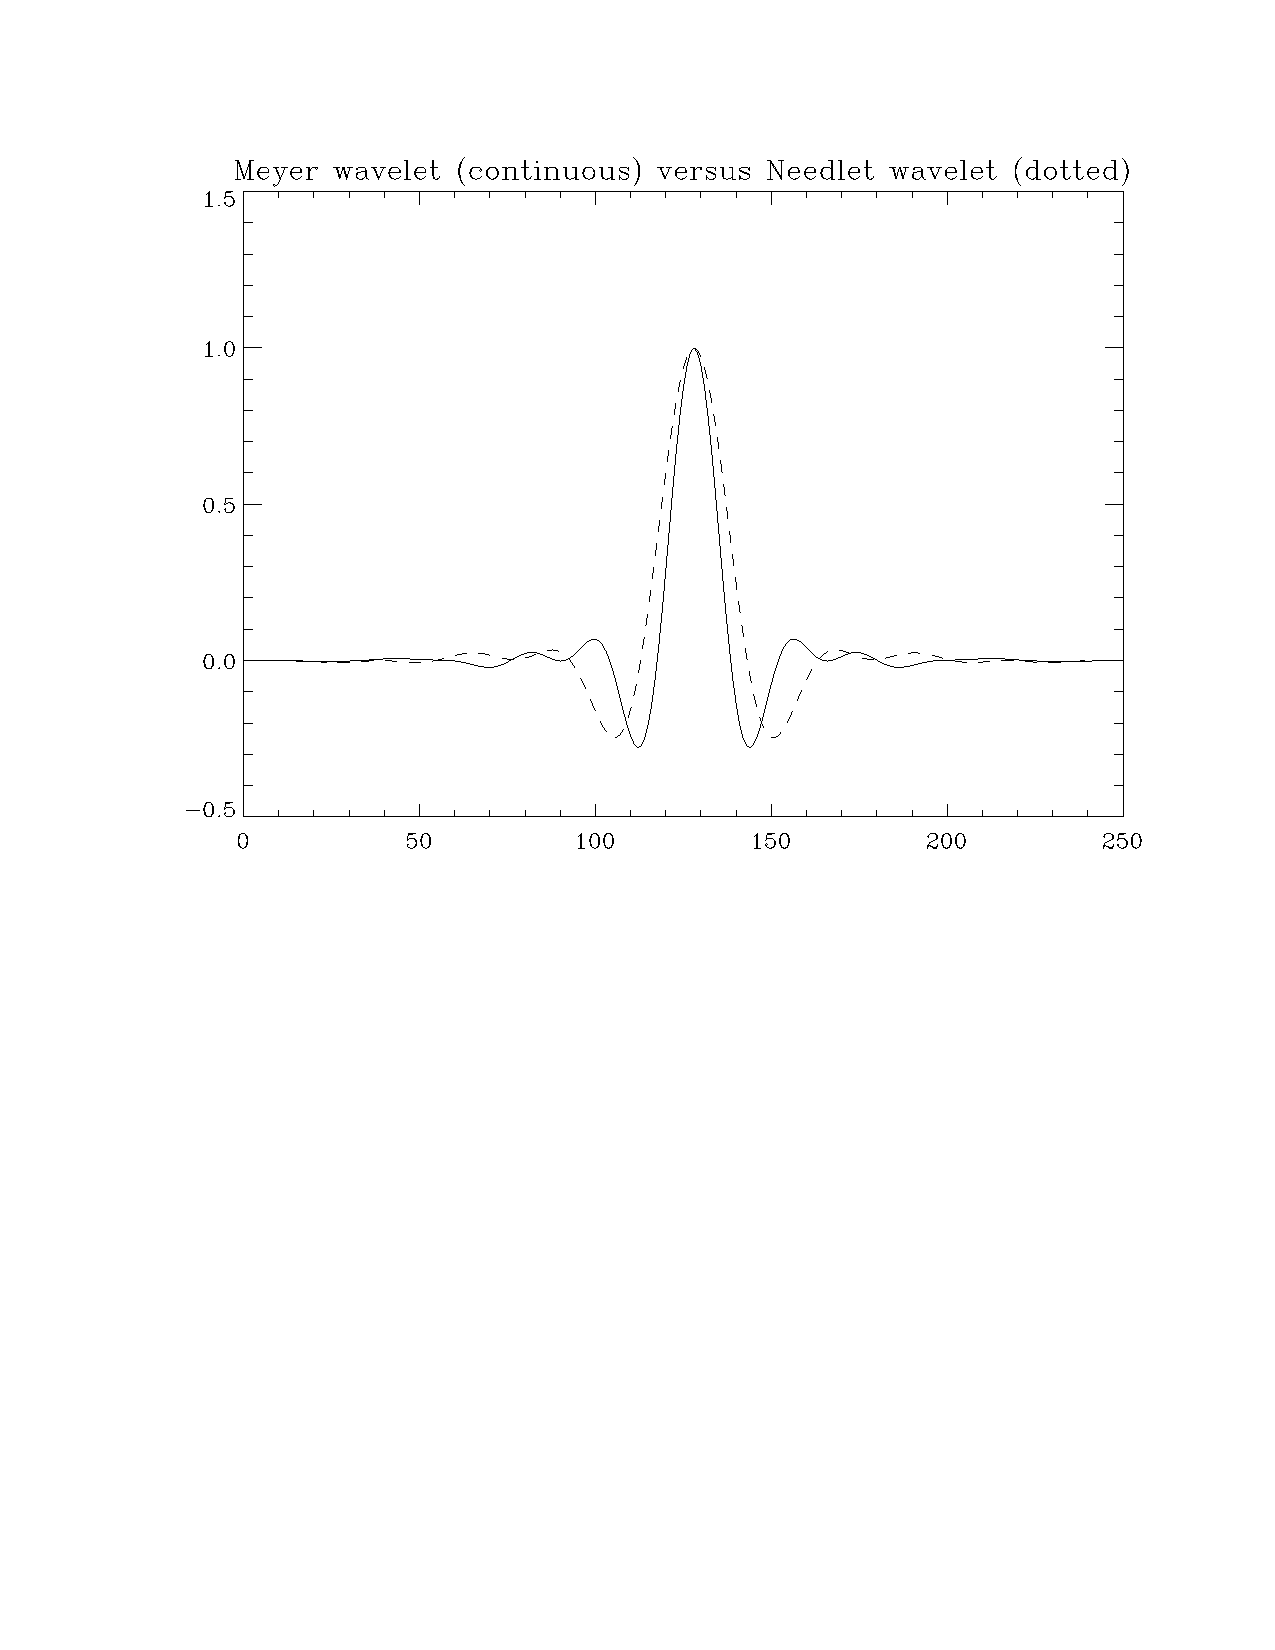
\includegraphics[width=7.5cm, trim= 2cm 14cm 2cm 2cm, clip=]{fig_meyerw_versus_needletw.pdf}
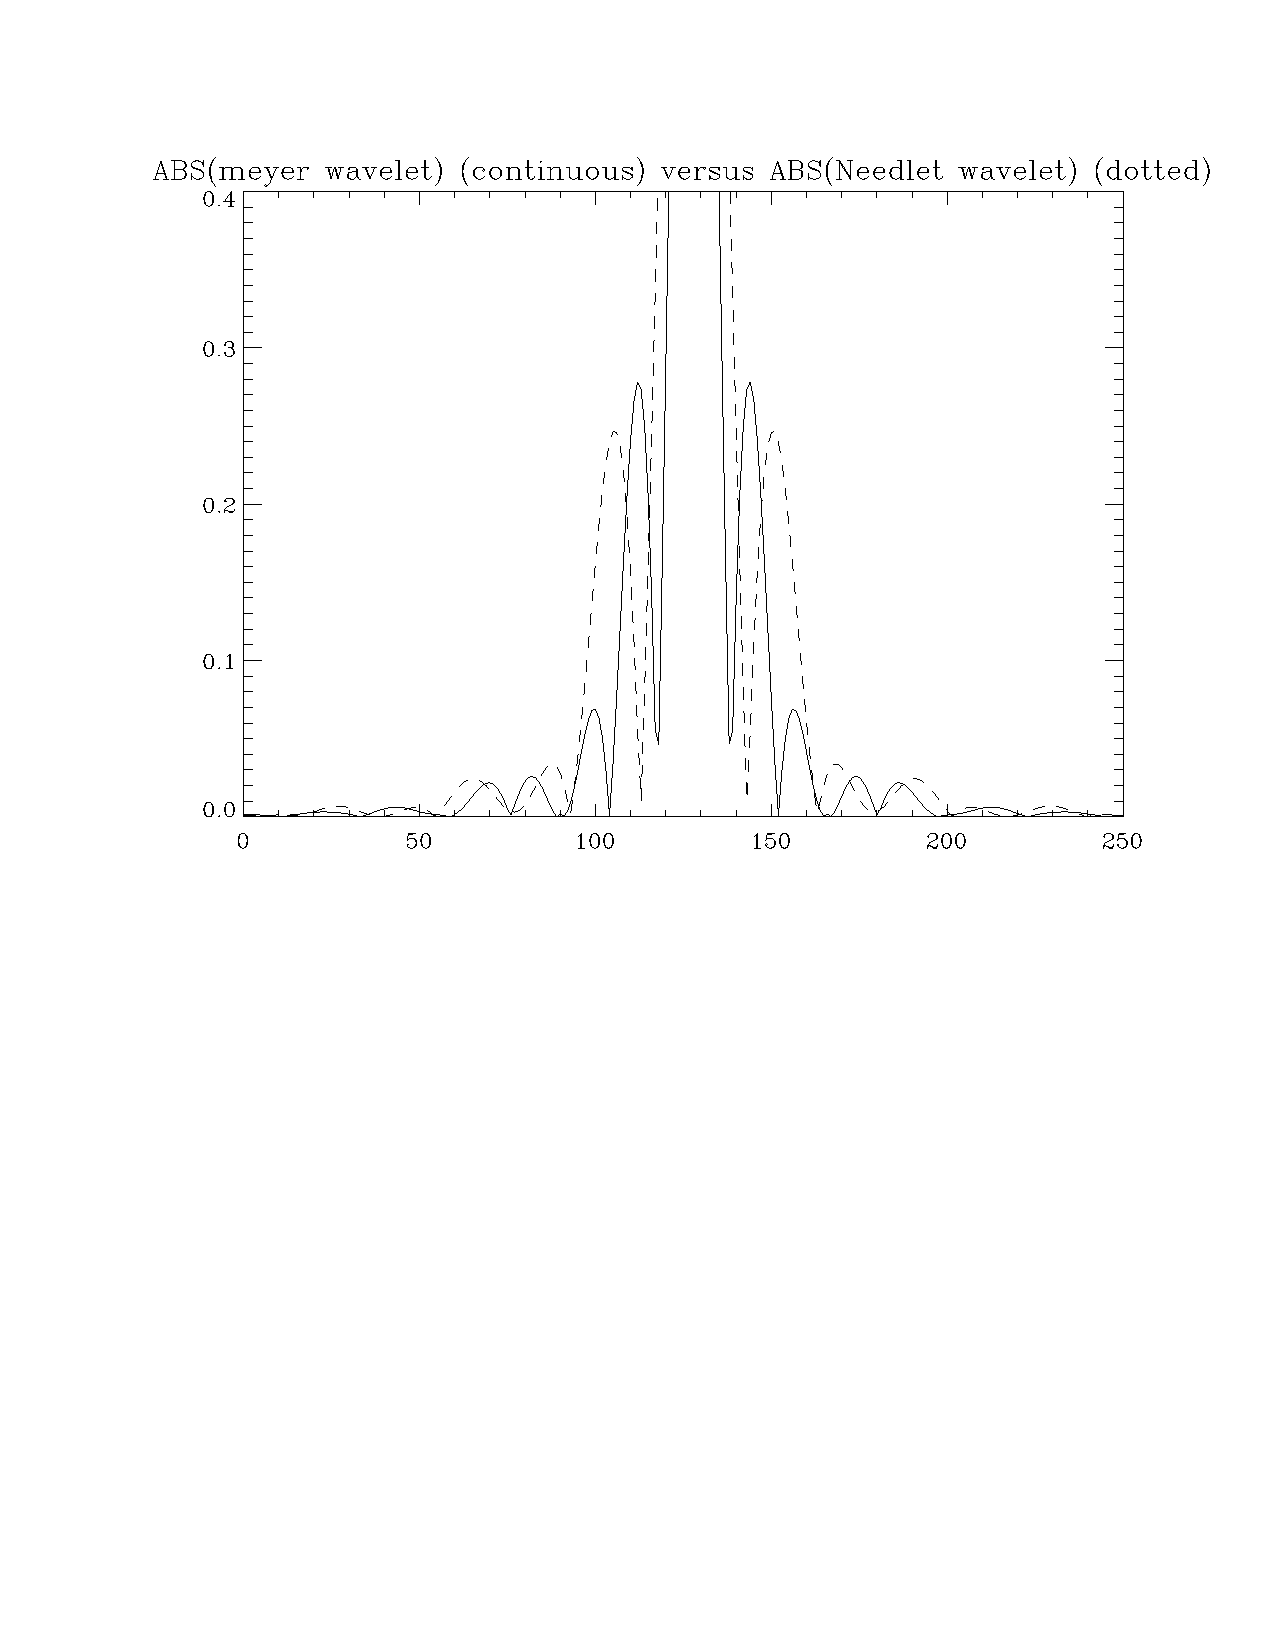
\includegraphics[width=7.5cm, trim= 2cm 14cm 2cm 2cm, clip=]{fig_absmeyerw_versus_absneedletw.pdf}
}}
}
\caption{Comparaison between spline, needlet, and Meyer wavelet functions on the sphere.}
\label{Figure:cmp_needlet}
\end{figure}

Any function with a cut-off frequency is a possible candidate. The 
B-spline function of order 3 \citep{starck2010,starck:sta06} leads to :
\begin{eqnarray}
{\hat{\phi}}_{l_c} [l,m] = \frac{3}{2} B_{3}  \left(  \frac{2l}{l_{c}} \right)
\end{eqnarray}
where $B_3(t)$ is the scaling function:
\begin{equation}
B_3(t) = \frac{1}{12}({\mid{t-2}\mid}^3 - 4 {\mid{t-1}\mid}^3 + 6 {\mid{t}\mid}^3 - 4 {\mid{t+1}\mid}^3 + {\mid{t+2}\mid}^3)
\end{equation}


In Fig.~\ref{fig_diff_uv_phi_psi} the spherical harmonics coefficients of the scaling function derived from a B$_3$-spline, 
and those of the associated wavelet function \eqref{wavelet}, are plotted as a function of $l$. Other functions such as 
Meyer wavelets or the needlet function \citep{marinucci08} can be used as well. 


Meyer and needlet wavelet functions have both a much better frequency localization than the wavelet function derived from the  B$_3$-spline,
and, as nothing is perfect, the price to pay is more oscillations in the direct space. To illustrate this, we 
show in Fig.~\ref{Figure:cmp_needlet} different wavelet functions.  Top left and right shows the respectively the spline and the needet wavelet function at a given scale. Fig.~\ref{Figure:cmp_needlet}~middle left shows a cut of the healpix face with contains the previous functions. Middle right is the same functions, but we have plotted the absolute value in order to better visualize their respective ringing.
As it can be seen, for wavelet functions with the same main lob, the needlet wavelet oscillate much more than the spline wavelet.  Fig.~\ref{Figure:cmp_needlet}~bottom left and right compares   Meyer and  needlet functions. They are relatively close and share
the same property of good frequency localization, but with more oscillations than the spline wavelet function.
Hence, the best wavelet choice certainly depends on the final applications. For statistical analysis, detection or restoration applications, 
we may prefer to use a wavelet which does not oscillate too much and with a smaller support, and the spline wavelet is clearly the 
correct choice. For spectral or bispectral analysis, where the frequency localization is fundamental, then Meyer or needlet shoud be 
preferred to the spline wavelet.


\begin{figure}[htb]
\vbox{
\centerline{
\hbox{
 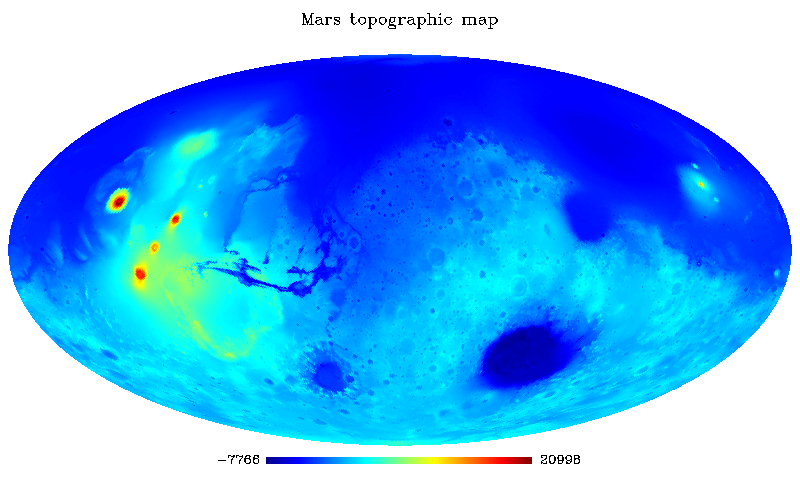
\includegraphics[width=7.5cm]{fig_mars.png}%[width=6.5cm,height=3.9cm]
 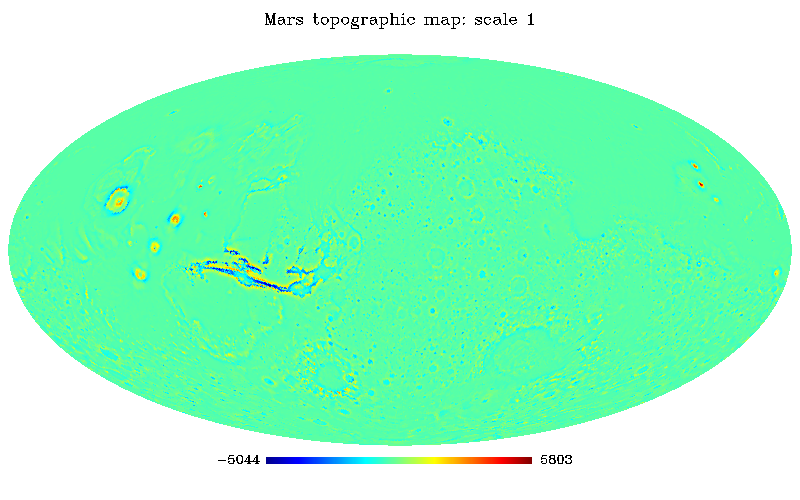
\includegraphics[width=7.5cm]{fig_mars_scale1.png}
}}
\centerline{
\hbox{
 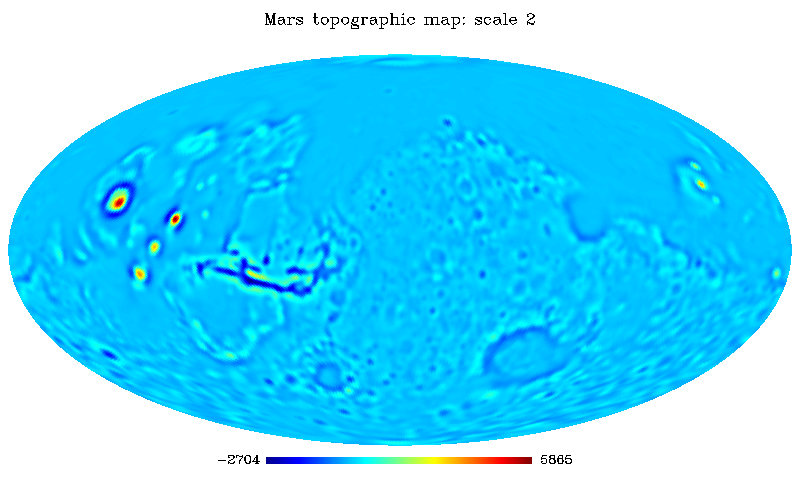
\includegraphics[width=7.5cm]{fig_mars_scale2.png}
 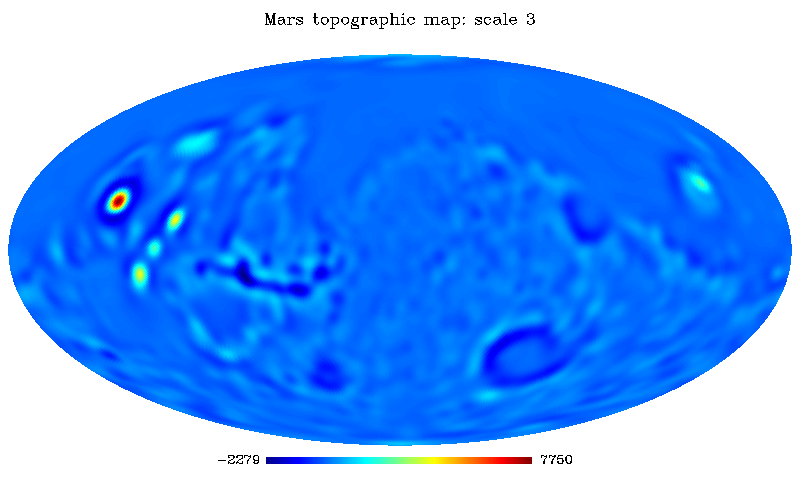
\includegraphics[width=7.5cm]{fig_mars_scale3.png}
}}
\centerline{
\hbox{
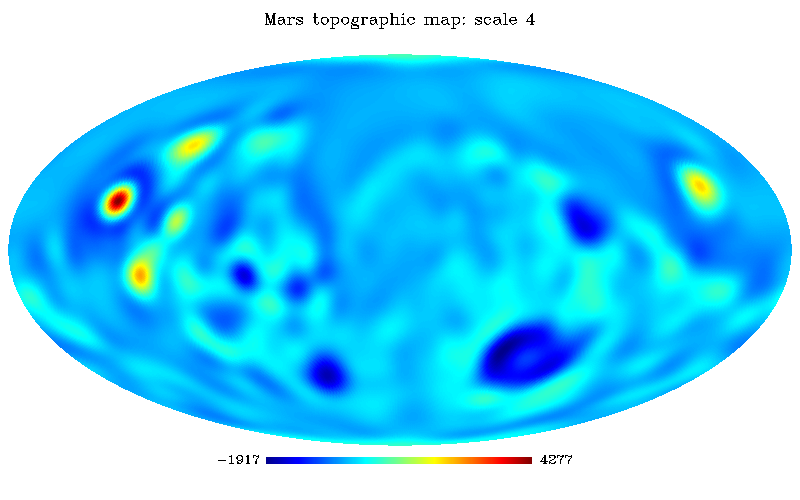
\includegraphics[width=7.5cm]{fig_mars_scale4.png}
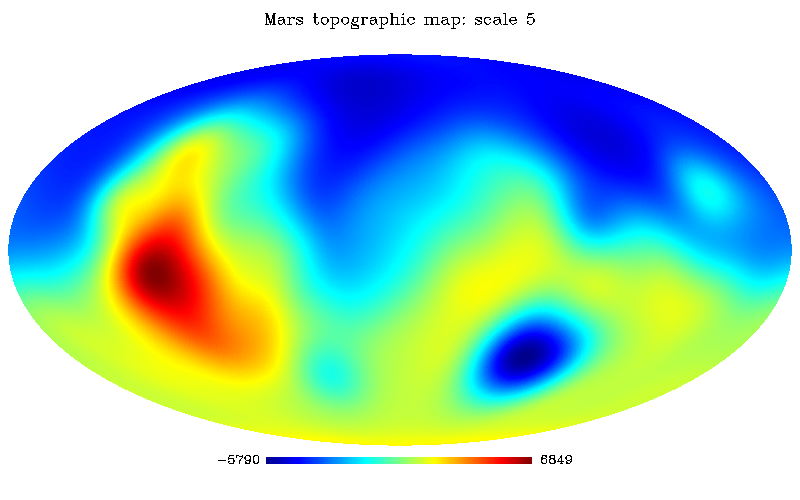
\includegraphics[width=7.5cm]{fig_mars_scale5.png}
}}
}
\caption{Mars topographic map and its UWTS (four wavelet detail scales and the scaling (smooth) band).}
\label{Figure:UWTS}
\index{data!Mars topography}
\end{figure}

The steps of the UWT on the sphere of a discrete image $X$ sampled from $f$ are summarized in Algorithm~\ref{algo_uwts}. 
If the wavelet function corresponds to the choice \eqref{wavelet}, Step 3 in this UWTS algorithm reduces to $w_{j+1} = c_{j} - c_{j+1}$.

% Their corresponding conjugate low pass and high pass filters $h$ and $g$ are plotted in Fig.~\ref{fig_diff_uv_ht_gt}. 

{\linespread{1}
\begin{algorithm}[h]
\caption{The Undecimated Wavelet Transform on the Sphere.}
\label{algo_uwts}
\noindent{\bf Task:} Compute the UWTS of a discrete $X$.\\
\noindent{\bf Parameters:} Data samples $X$ and number of of wavelet scales $J$.\\  
\noindent{\bf Initialization:} 
\begin{itemize}
\item $c_0=X$.
\item Compute the B$_3$-spline scaling function and derive $\hat{\psi}$, $\widehat{H}$ and $\widehat{G}$ numerically.
\item Compute the corresponding spherical harmonics transform of $c_0$.
\end{itemize}
\For{$j=0$ to $J-1$} {
\begin{enumerate}[1.]
\item Compute the spherical harmonics transform of the scaling coefficients:  $\hat{c}_{j+1}=\hat{c}_j\widehat{H}_{j}$.
\item Compute the inverse spherical harmonics transform of $\hat{c}_{j+1}$ to get $c_{j+1}$.
\item Compute the spherical harmonics transform of the wavelet coefficients:  $\hat{w}_{j+1}=\hat{c}_j\widehat{G}_{j}$.
\item Compute the inverse spherical harmonics transform of $\hat{w}_{j+1}$ to get $w_{j+1}$.
\end{enumerate}
}
\noindent{\bf Output:} ${\cal W}=\{w_1, w_2, \dots, w_{J}, c_{J}\}$ the UWTS of $X$.
\end{algorithm}
}

Fig.~\ref{Figure:UWTS} shows the Mars topographic map (top left)
\footnote{The Mars Orbiter Laser Altimeter (MOLA) generated altimetry profiles used to create global topographic maps. The MOLA instrument stopped acquiring altimetry data on June 30, 2001, and after that operated in passive radiometry mode until the end of the Mars Global Surveyor mission. MOLA data sets are produced by the MOLA Science Team and archived by the PDS Geosciences Node.} and its wavelet transform, using five scales (four wavelet scales + coarse scale). The sum of the five scales reproduces exactly the original image.
\index{Mars Orbiter Laser Altimeter}

\subsubsection{Inverse Transform}

If the wavelet is the difference between two resolutions, a straightforward reconstruction of an image from its wavelet coefficients ${\cal W} = \{w_1,\dots, w_{J}, c_{J}\}$ is: 

\begin{eqnarray}
 c_{0}(\theta, \vartheta) = c_{J}(\theta, \vartheta) + \sum_{j=1}^J  w_j(\theta, \vartheta) .
\end{eqnarray}
This reconstruction formula is the same as with the 2D undecimated isotropic wavelet algorithm (i.e. with \`a trous agorithm).

\begin{figure}[htb]
\vbox{
\centerline{
\hbox{
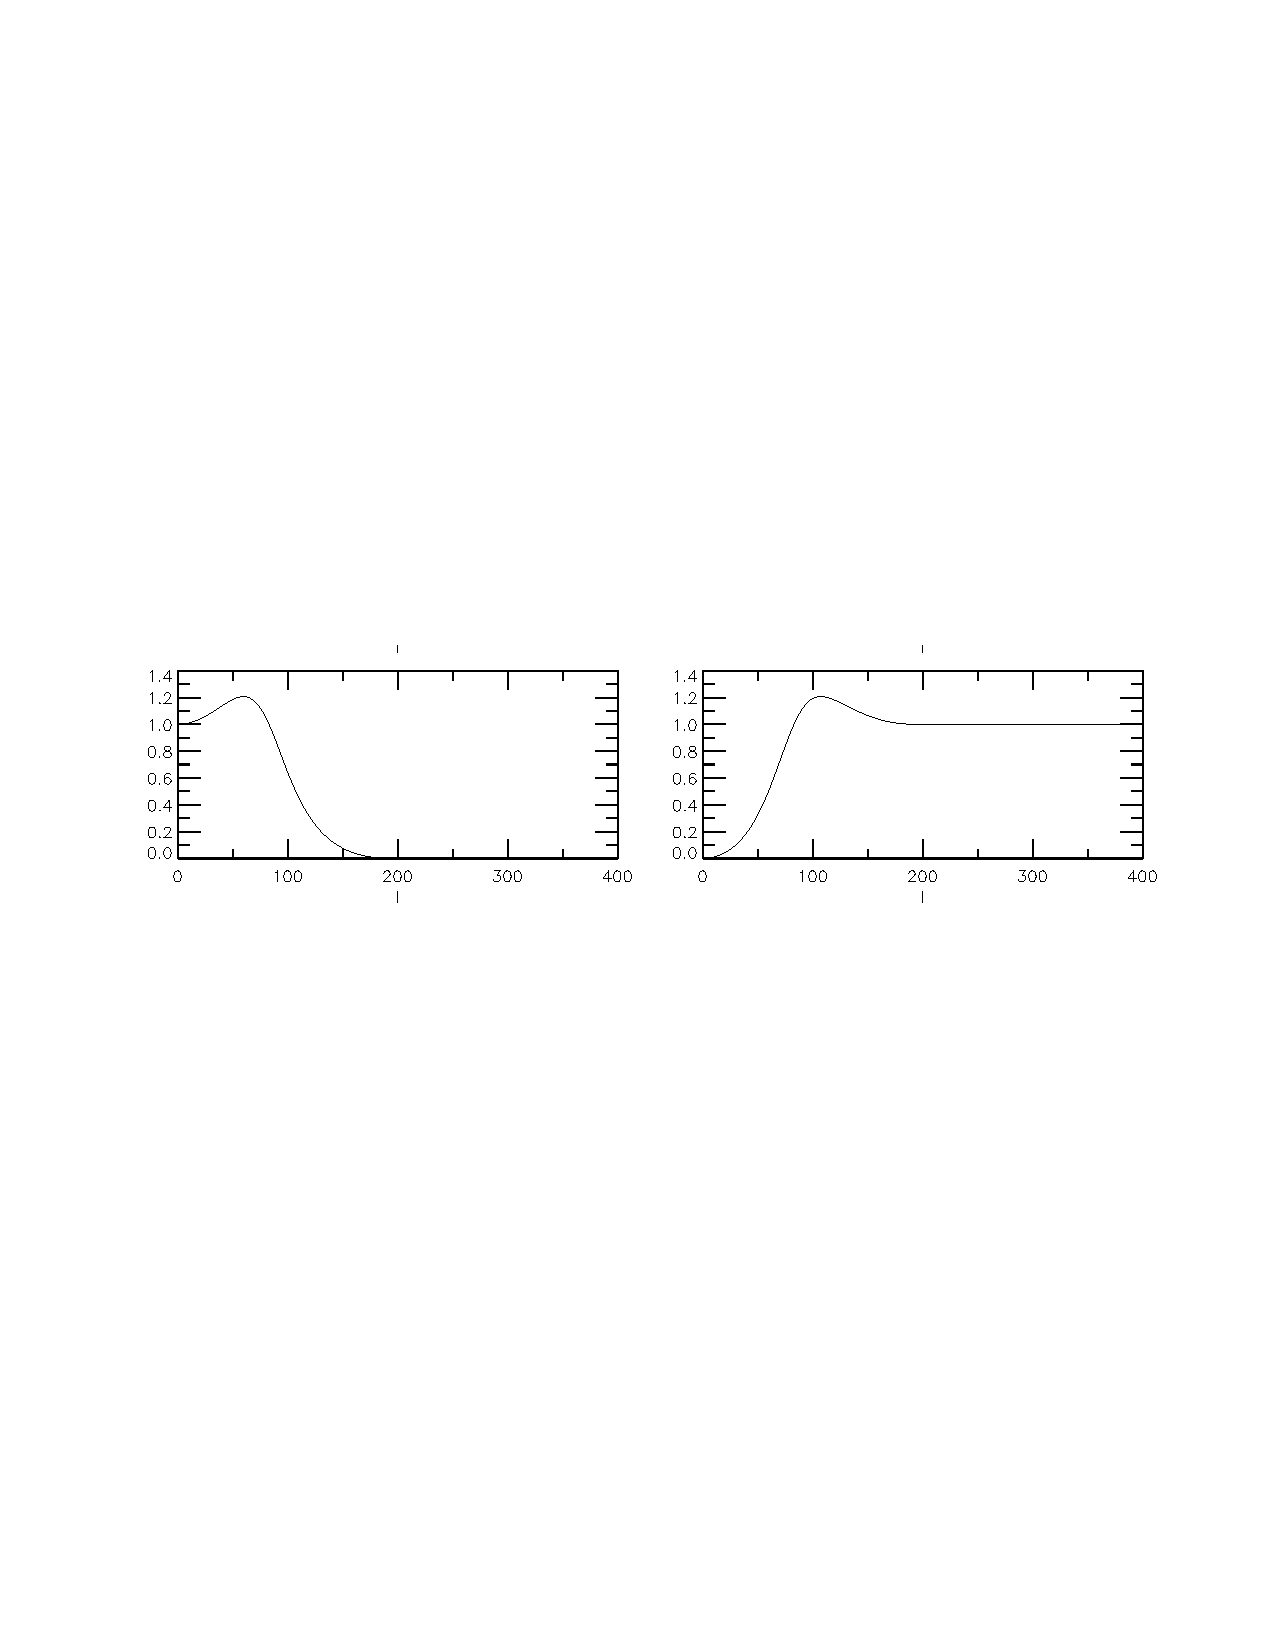
\includegraphics[width = 15cm, height = 5cm]{fig_sphere_filterbank2.pdf} 
% 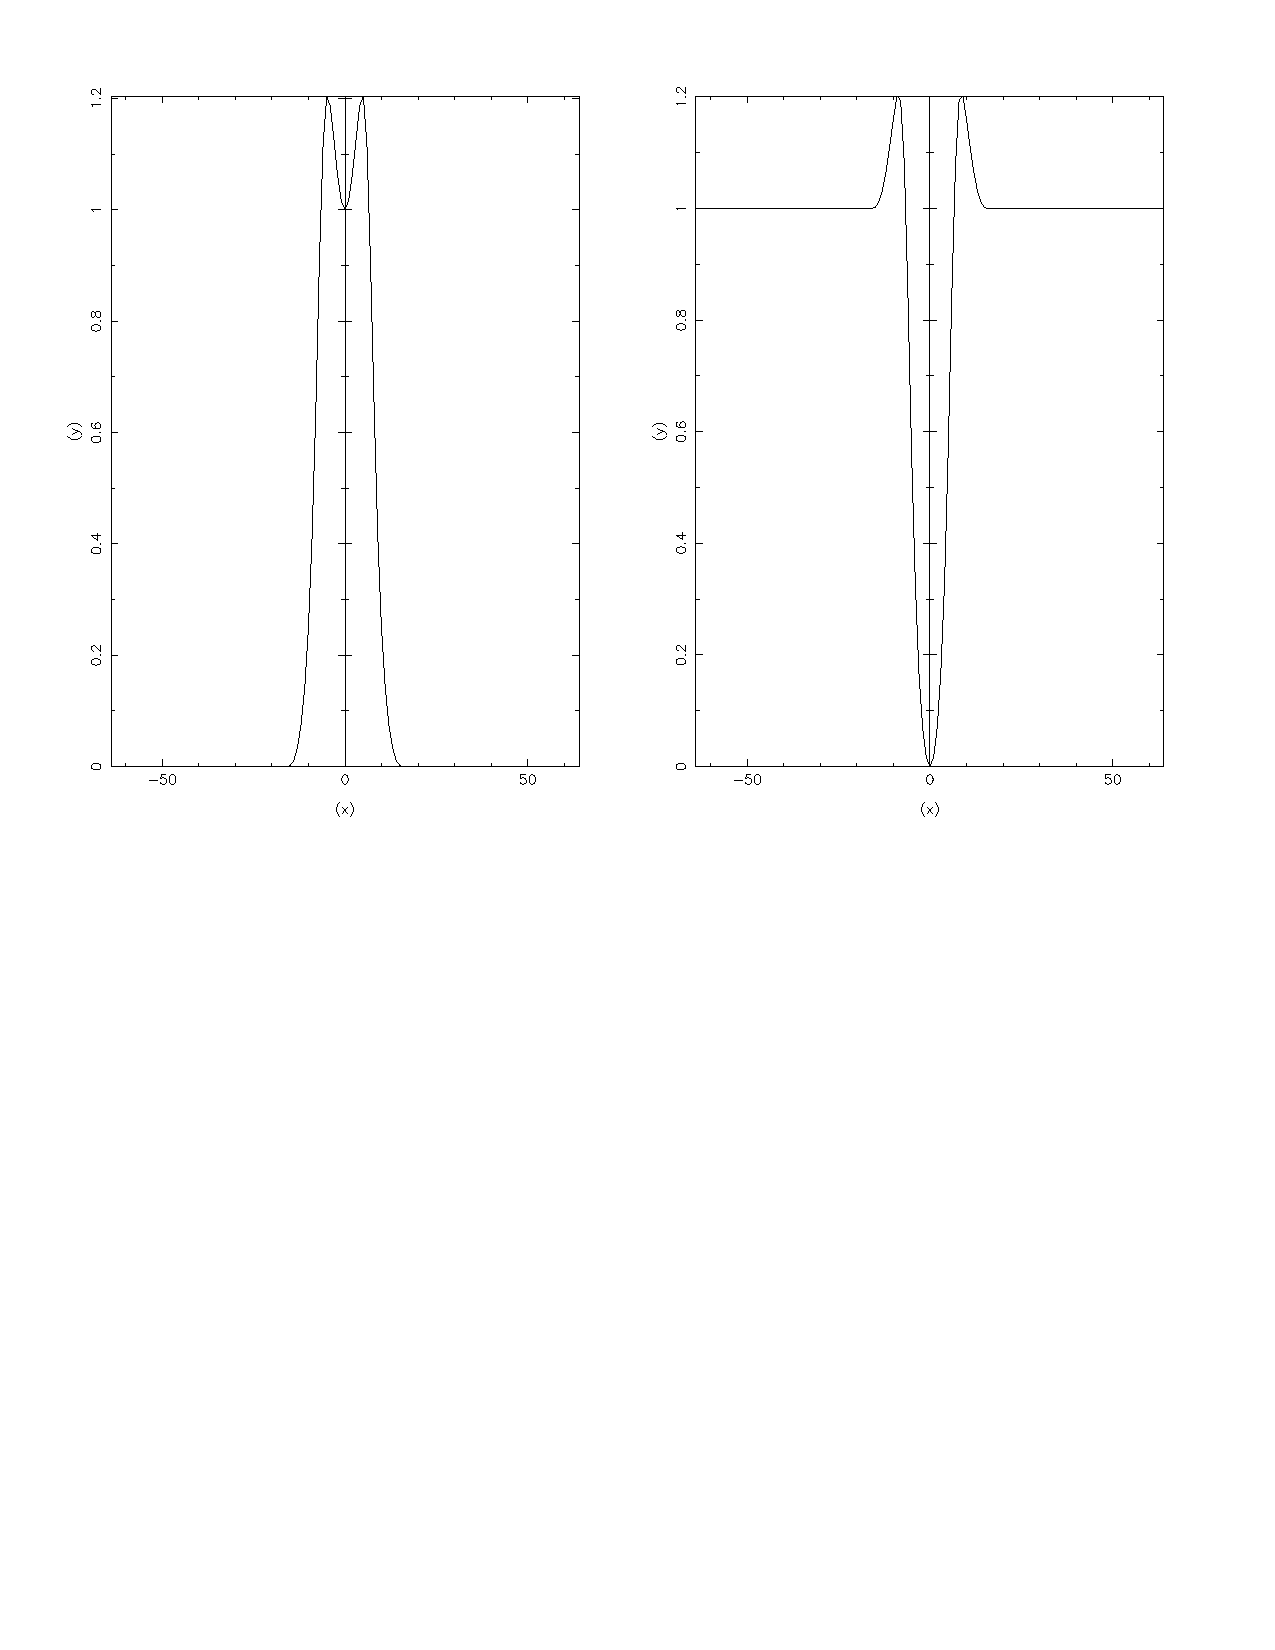
\includegraphics[width=14.5cm,height=5cm]{ch1_diff_uv_ht_gt.pdf}
}}}
\caption{On the left, the filter $\hat{\tilde{h}}$, and on the right the 
filter $\hat{\tilde{g}}$.}
\label{fig_diff_uv_ht_gt}
\end{figure}

But since the transform is redundant there is actually no unique way to reconstruct an image from its coefficients see~\citep{starck:sta06}. Indeed, using the relations:
\begin{eqnarray}
\begin{split}
\hat c_{j+1}[l,m] = \widehat H_{j} [l,m]  \hat c_{j} [l,m] \\
\hat w_{j+1}[l,m] = \widehat G_{j} [l,m] \hat c_{j} [l,m] 
\end{split}
\end{eqnarray}
a least-squares estimate of $c_j$ from $c_{j+1}$ and $w_{j+1}$ gives:
\begin{eqnarray}
\hat{c}_{j}   = \hat{c}_{j+1}  {\widehat {\tilde H}}_{j}   + \hat{w}_{j+1}  {\widehat {\tilde G}}_{j} ~,
\end{eqnarray}
where the dual filters $\tilde h$ and $\tilde g$ satisfy:
\begin{eqnarray}
\label{eqnht} 
\begin{split}
{\widehat {\tilde H}}_j =  \sqrt{\frac{4\pi}{2l+1} } {\hat {\tilde h}}_j & = {\widehat H}_{j}^* /
\parenth{\big|{\widehat H}_{j}\big|^2 + \big|{\widehat G}_j\big|^2} \\
{\widehat {\tilde G}}_j =  \sqrt{\frac{4\pi}{2l+1} } {\hat {\tilde g}}_j & = {\widehat G}_{j}^* /
\parenth{\big|{\widehat H}_j\big|^2 + \big|{\widehat G}_j\big|^2} .
\end{split}
\end{eqnarray}
For the scaling function which is a B$_3$-spline function and a wavelet taken as the difference between two resolutions,
the corresponding conjugate low pass and high pass filters $\widehat {\tilde H}$ and $\widehat {\tilde G}$ are plotted in Fig.~\ref{fig_diff_uv_ht_gt}. 
The reconstruction algorithm is given in Algorithm~\ref{algo_iuwts}.

{\linespread{1}
\begin{algorithm}[h]
\caption{Inverse UWT on the sphere.}
\label{algo_iuwts}
\noindent{\bf Task:} Reconstruct an image from its UWTS coefficients.\\
\noindent{\bf Parameters:} UWTS coefficients ${\cal W}=\{w_1, w_2, \dots, w_{J}, c_{J}\}$.\\
\noindent{\bf Initialization:}
\begin{itemize}
\item Compute the B$_3$-spline scaling function and derive $\hat{\psi}$, $\widehat{H}$, $\widehat{G}$, $\widehat{\tilde H}$ and $\widehat{\tilde G}$ numerically.
\item Compute the spherical harmonics transform of $c_J$ to get ${\hat c}_J$.
\end{itemize}
\For{$j=J-1$ to $0$, with step $=-1$} {
\begin{enumerate}[1.]
\item Compute the spherical harmonics transform of the wavelet coefficients $w_{j+1}$ to get $\hat{w}_{j+1}$.
\item Multiply $\hat{c}_{j+1}$ by ${\widehat {\tilde H}}_{j}$.
\item Multiply $\hat{w}_{j+1}$ by ${\widehat {\tilde G}}_{j}$.
\item Get the spherical harmonics of $\hat{c}_j=\hat{c}_{j+1}+\hat{w}_{j+1}$.
\end{enumerate}
}
Compute The inverse Spherical Harmonics transform of $\hat c_0$.\\
\noindent{\bf Output:} $c_0$ is the inverse UWT on the sphere.
\end{algorithm}

\begin{figure}[htb]
\centerline{
\hbox{
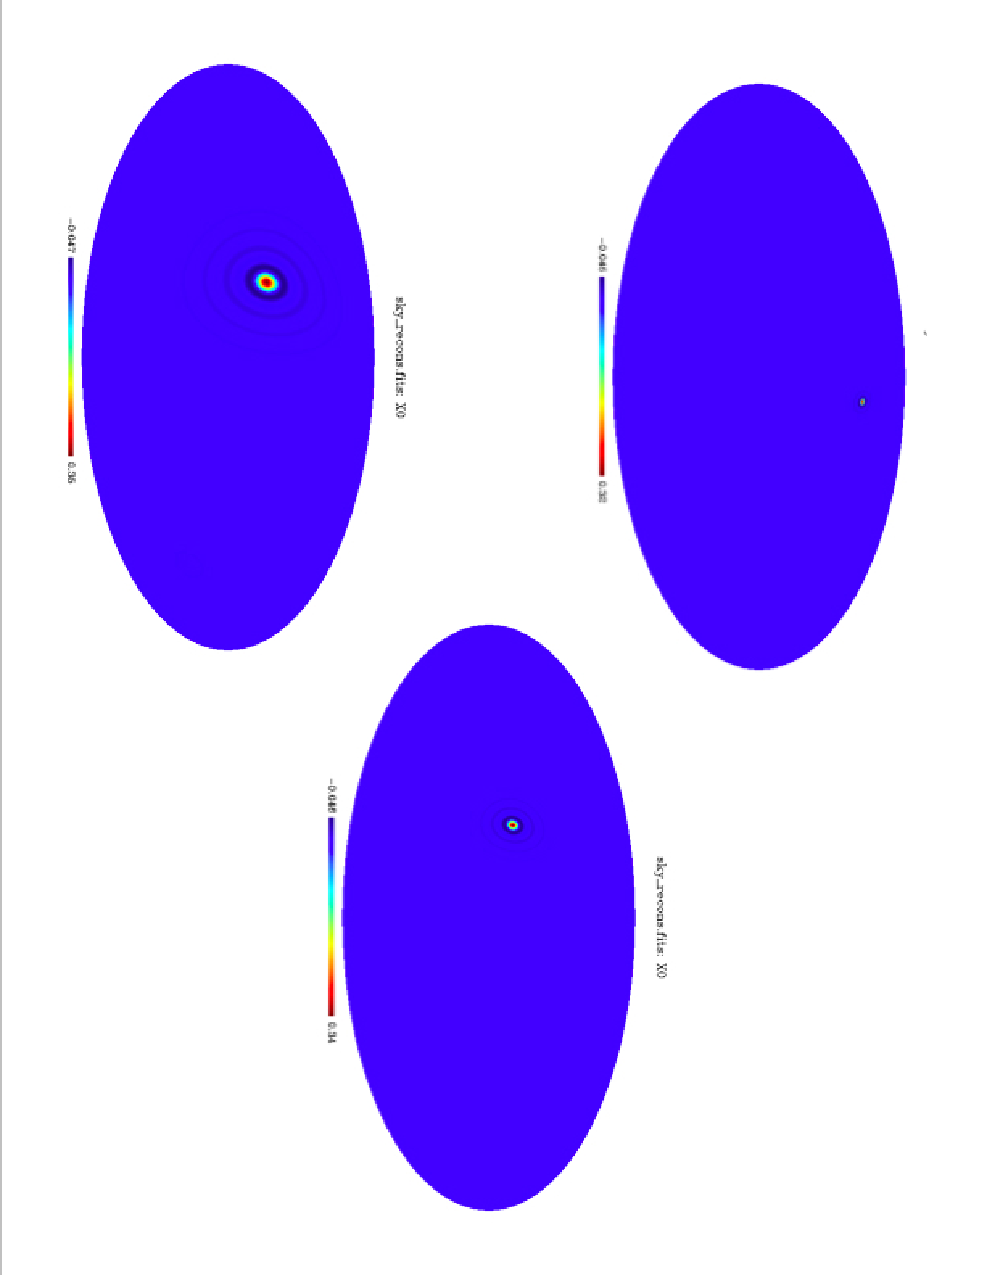
\includegraphics[width = 12cm,angle = 90]{fig_backwt_sphere.pdf}
}}
\caption{Reconstruction from a single wavelet coefficient at different scales. Each map is obtained by setting all wavelet coefficients to zero but one, and by applying an inverse UWTS. Depending on the position and scale of the non-zero coefficient, the reconstructed map shows an isotropic feature 
at different scales and positions.}
\label{Figure:back_wt}
\end{figure}
}
Fig.~\ref{Figure:back_wt} shows the reconstruction by setting all wavelet coefficients but one at different scales and positions. 
Depending on the position and scale of the non-zero coefficient, the reconstructed map shows an isotropic feature at different scales and positions.
 

%-------------------------

\subsection{Isotropic Pyramidal Wavelet Transform on the Sphere}
\index{wavelet!pyramidal transform}
\index{sphere!pyramidal wavelet}

\subsubsection{Forward Transform}
In the previous algorithm, no down-sampling is performed and each scale of the wavelet decomposition has the same number of pixels 
as the original data set. Therefore the number of pixels in the decomposition is equal to the number of pixels in the data multiplied 
by the number of scales. For some applications, we may prefer to introduce a decimation in the decomposition so as to reduce the 
required memory size and the computation time. This can be done easily by using a specific property of the chosen scaling function.
Indeed, since we are considering here a scaling function with an initial cut-off $l_c$ in spherical harmonic multipole number $l$, 
and since the actual cut-off is reduced by a factor of two at each step, the number of significant spherical harmonics coefficients 
is then reduced by a factor of four after each convolution with the low pass filter $h$. Therefore, we need less pixels in the direct 
space when we compute the inverse spherical harmonics transform. Using the HEALPix pixelization scheme \citep{pixel:healpix}, 
this can be done easily by dividing by 2 the $N_{\mathrm{side}}$ parameter when calling the inverse spherical harmonics transform routine.
The pyramidal wavelet transform on the sphere algorithm is given in Algorithm~\ref{algo_pwts}.

{\linespread{1}
\begin{algorithm}[h]
\caption{Pyramidal wavelet transform on the sphere.}
\label{algo_pwts}
\noindent{\bf Task:} Compute the pyramidal WT on the sphere of a discrete image $X$.\\
\noindent{\bf Parameters:} Data $X$ and number of of wavelet scales $J$.\\
\noindent{\bf Initialization:} 
\begin{itemize}
\item $c_0=X$.
\item Compute the B$_3$-spline scaling function and derive $\hat{\psi}$, $\widehat{H}$ and $\widehat{G}$ numerically.
\item Compute the corresponding spherical harmonics transform of $c_0$.
\end{itemize}
\For{$j=0$ to $J-1$} {
\begin{enumerate}[1.]
\item Compute the spherical harmonics transform of the scaling coefficients:  $\hat{c}_{j+1}=\hat{c}_j\widehat{H}_{j}$.
\item Compute the inverse spherical harmonics transform of $\hat{c}_{j+1}$ to get $c_{j+1}$.
\item Down-sample $c_{j+1}$, since its support in the spherical harmonic domain has been divided by two.
\item Compute the spherical harmonics transform of the wavelet coefficients:  $\hat{w}_{j+1}=\hat{c}_j\widehat{G}_{j}$.
\item Compute the inverse spherical harmonics transform of $\hat{w}_{j+1}$ to get $w_{j+1}$.
\end{enumerate}
}
\noindent{\bf Output:} ${\cal W}=\{w_1, w_2, \dots, w_{J}, c_{J}\}$ the Pyramidal WT on sphere of $X$.
\end{algorithm}
}

\begin{figure}[htb]
\vbox{
\centerline{
\hbox{
 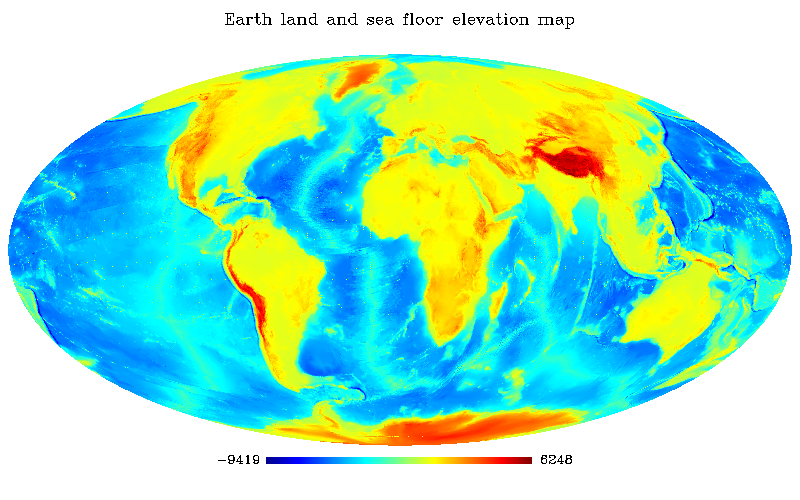
\includegraphics[width=7.5cm]{fig_earth_elevation.png}%[width=6.5cm,height=3.9cm]
 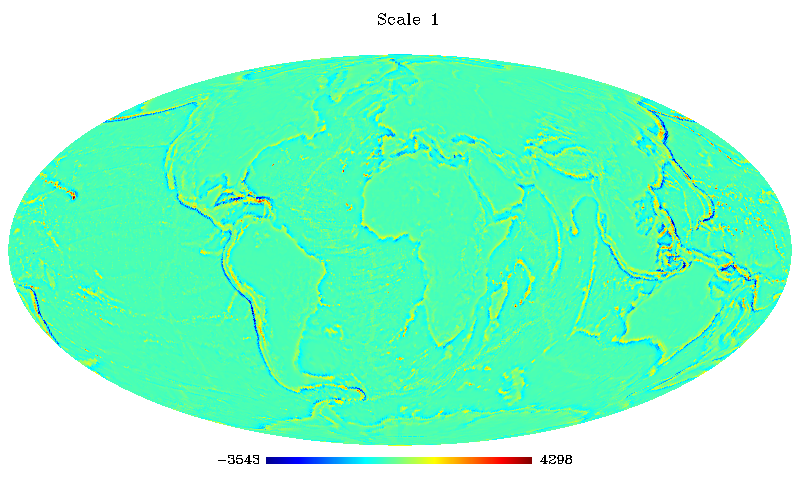
\includegraphics[width=7.5cm]{fig_earth_scale_1.png}
}}
\centerline{
\hbox{
 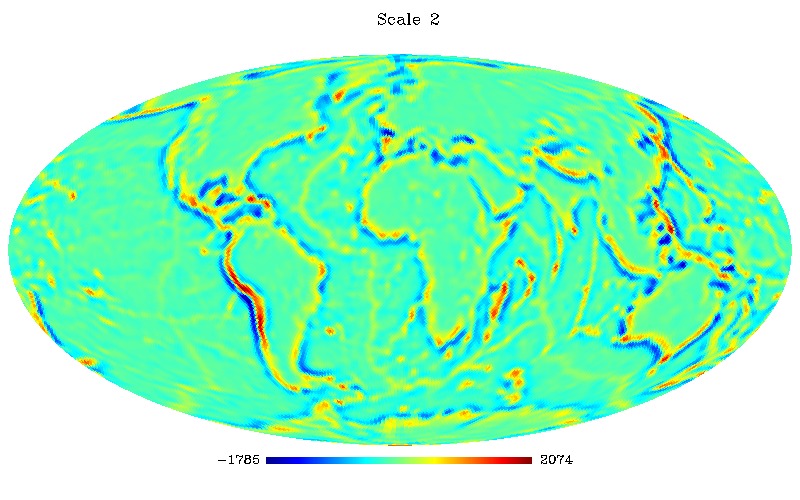
\includegraphics[width=7.5cm]{fig_earth_scale_2.png}
 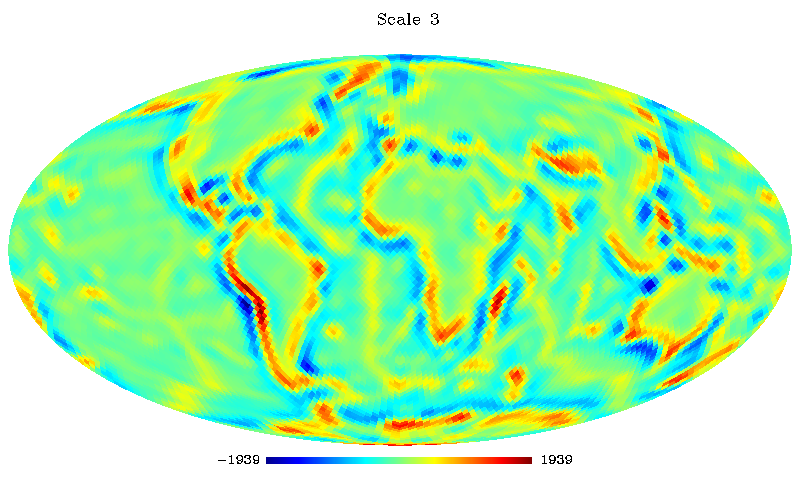
\includegraphics[width=7.5cm]{fig_earth_scale_3.png}
}}
\centerline{
\hbox{
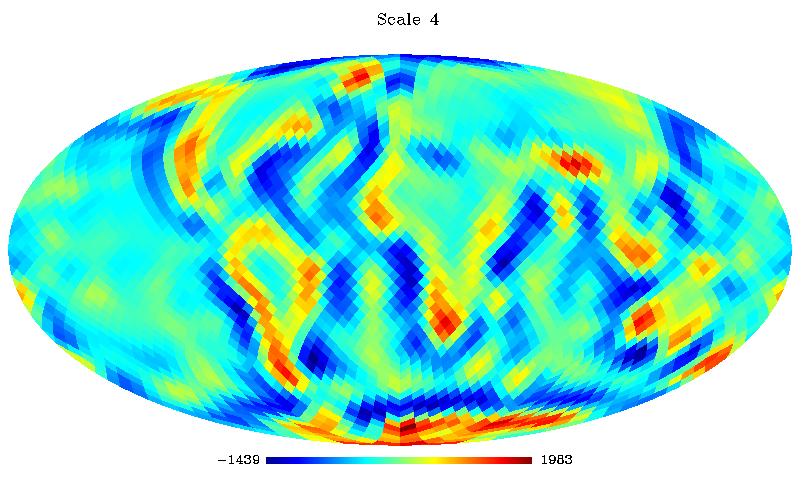
\includegraphics[width=7.5cm]{fig_earth_scale_4.png}
\includegraphics[width=7.5cm]{fig_earth_scale_5.png}
}}
}
\caption{Pyramidal wavelet transform on the sphere.}.
\label{Figure:PWTS}
\end{figure}

Fig.~\ref{Figure:PWTS} shows an Earth image and its pyramidal wavelet transform (PWTS) using five scales.
As the scale number increases (i.e.\ the resolution decreases), the pixel size becomes larger. The data are 
land and sea-floor elevations obtained from the ETOPO5 5-minute gridded elevation data set. A thorough explanation 
of the data set is provided at \texttt{www.ngdc.noaa.gov} \footnote{The ETOPO5 data are credited to ``Data Announcement 88-MGG-02, 
Digital relief of the Surface of the Earth. NOAA, National Geophysical Data Center, Boulder, Colorado, 1988''. The HEALPix image 
is available at \texttt{http://astro.ic.ac.uk/$\sim$pdineen/earth/index.html\#earthmap}.}.


%\newpage
\subsubsection{Inverse Transform}
 
This reconstruction is not as straightforward as in the undecimated case, since the different scales do not have the same resolution.
For each resolution level, we have to up-sample the scaling band before co-adding it to the wavelet coefficients. Algorithm \ref{algo_ipwts} describes this.
{\linespread{1}
\begin{algorithm}[h]
\caption{Inverse Pyramidal Wavelet Transform on the sphere.}
\label{algo_ipwts}
{\bf Task:} Reconstruct an image from its pyramidal WT on the sphere.\\
\noindent{\bf Parameters:} Pyramidal WT coefficients ${\cal W}=\{w_1, w_2, \dots, w_{J}, c_{J}\}$.\\
{\bf Initialization:}
\begin{itemize}
\item Compute the B$_3$-spline scaling function and derive $\hat{\psi}$, $\widehat{H}$, $\widehat{G}$, $\widehat{\tilde H}$ and $\widehat{\tilde G}$ numerically.
\item Compute the spherical harmonics transform of $c_J$ to get ${\hat c}_J$.
\end{itemize}
\For{$j=J-1$ to $0$} {
\begin{enumerate}[1.]
\item Upsample $c_{j+1}$ to the resolution of $c_j$.
\item Compute the spherical harmonics transform of the wavelet coefficients $w_{j+1}$ to get $\hat{w}_{j+1}$.
\item Multiply $\hat{c}_{j+1}$ by ${\widehat {\tilde H}}_{j}$.
\item Multiply $\hat{w}_{j+1}$ by ${\widehat {\tilde G}}_{j}$.
\item Get the spherical harmonics of $\hat{c}_j=\hat{c}_{j+1}+\hat{w}_{j+1}$.
\end{enumerate}
}
Compute The inverse spherical harmonics transform of $\hat c_0$.\\
\noindent{\bf Output:} $c_0$ is the inverse pyramidal WT on the sphere.
\end{algorithm}
}
  
The wavelet transform on the sphere and its pyramidal version have both a reconstruction operator, 
so they are very well designed for any restoration application when the data contains isotropic features. 
In the following, we present other transforms on the sphere more adapted to the analysis of anisotropic features.





\section{Ridgelet and Curvelet Transform on the Sphere (CTS) }
\label{sect_cur}
\subsection{Introduction.}
\index{curvelet}
\index{curvelet!sphere}
\index{sphere!curvelet}

The 2D curvelet transform, proposed in \citep{cur:donoho99,starck:sta01_3,starck:sta02_3}, enables the directional analysis of an image 
in different scales. The fundamental property of the curvelet transform is to analyze the data with functions of length about $2^{-j/2}$ 
for the $j^{\textrm{th}}$ sub-band $[2^j, 2^{j+1}]$ of the two dimensional wavelet transform. Following the implementation described 
in \citep{starck:sta01_3,starck:sta02_3}, the data first undergoes an Isotropic Undecimated Wavelet Transform (i.e. \og{}\`a trous \fg{} algorithm). 
Each scale $j$ is then decomposed into smoothly overlapping blocks of side-length $B_j$ pixels in such a way that the overlap between two
vertically adjacent blocks is a rectangular array of size $B_j \times B_j/2$. And finally, the ridgelet transform \citep{cur:candes99_1} is 
applied on each individual block. Recall that the ridgelet transform precisely amounts to applying a 1-dimensional wavelet transform to the
slices of the Radon transform. More details on the implementation of the digital curvelet transform can be found in \citep{starck:sta01_3,starck:sta02_3}.
It has been shown that the curvelet transform could be very useful for the detection and the discrimination of non-Gaussianity in CMB \citep{starck:sta02_4}.
The curvelet transform is also redundant, with a redundancy factor of $16J+1$ whenever $J$ scales are employed. Its complexity scales like 
that of the ridgelet transform that is as $O(n^2 \log_2n)$. The curvelet transform was shown to sparsely represent anisotropic structures and smooth curves and edges of different lengths.

\subsection{Ridgelets and Curvelets on the Sphere.}
\index{curvelet transform}
The Curvelet transform on the sphere (CTS) can be similar to the 2D digital curvelet transform, but replacing the \og{}\`a trous \fg{} algorithm 
by the Isotropic Wavelet Transform on the Sphere previously described. The CTS algorithm consists in the following three steps which 
we describe in more details next.
\begin{itemize}
\item {\it Isotropic Wavelet Transform on the Sphere.}  
\item {\it Partitioning.} Each scale is decomposed into blocks of an appropriate scale (of side-length $\sim2^{-s}$),using the HEALPix pixelization.
\item {\it Ridgelet Analysis.} Each square is analyzed via the discrete ridgelet transform.
\end{itemize}
We now describe these three steps.

\subsubsection{Partitioning Using the HEALPix Representation}

 \begin{figure}
\centerline{
\hbox{
\includegraphics[width=15cm]{fig_flowgraph_ridgelet_sphere.pdf}
% \includegraphics[width=13.6cm,height=8cm]{fig_flowgraph_ridgelet_sphere.pdf}
}}
\caption{Flowgraph of the ridgelet transform on the sphere.}
\label{Figure:rid_sphere}
\end{figure}

The HEALPix representation is a curvilinear hierarchical partition of the sphere into quadrilateral pixels 
of exactly equal area but with varying shape. The base resolution divides the sphere into 12 quadrilateral 
faces of equal area placed on three rings around the poles and equator. Each face is subsequently divided 
into $N_{\mathrm{side}}^{2}$ pixels following a quadrilateral multiscale tree structure (see Fig.~\ref{pixelhealpix}). 
The pixel centers are located on iso-latitude rings, and pixels from the same ring are equispaced in azimuth. 
This is critical for computational speed of all operations involving the evaluation of spherical harmonics transforms, 
including standard numerical analysis operations such as convolution, and power spectrum estimation. 

An important geometrical feature of the HEALPix sampling grid is the hierarchical quadrilateral tree structure. 
This defines a natural one-to-one mapping of the sphere sampled according to the HEALPix grid, into twelve 
flat images, on all scales. It is then easy to partition a spherical map using HEALPix into quadrilateral blocks 
of a specified size. One first extracts the twelve base-resolution faces, and each face is then decomposed into 
overlapping blocks of the specified size. This decomposition into blocks is an essential step of the traditional 
flat 2D curvelet transform. Based on the reversible warping of the sphere into a set of flat images made possible 
by the HEALPix sampling grid, the ridgelet and curvelet transforms can be extended to the sphere. 

With the decomposition into blocks described above, there is no overlap between neighboring blocks belonging 
to different base-resolution faces. This may result for instance in blocking effects in denoising experiments 
via nonlinear filtering. It is possible to overcome this difficulty in some sense by working simultaneously 
with various rotations of the data with respect to the sampling grid. This will average out undesirable effects 
at edges between base resolution faces. 

\subsubsection*{Ridgelet transform}
\index{ridgelet}
\index{ridgelet!sphere}
\index{sphere!ridgelet}
\index{Radon transform}

Once the partitioning is performed, the standard 2D ridgelet transform described in \citep{starck:sta02_3} is applied in each individual block :
\begin{enumerate}
\item Compute the 2D Fourier transform.
\item Extract lines going through the origin in the frequency plane.
\item Compute the 1D inverse Fourier transform of each line. We get the Radon transform.
\item Compute the 1D wavelet transform of the lines of the Radon transform.
\end{enumerate}
The first three steps correspond to a Radon transform method called the {\it linogram}. Other implementations of the Radon transform, such as 
the {\it Slant Stack Radon Transform} \citep{cur:donoho_02}, can be used as well, as long as they offer an exact reconstruction.
   
Fig.~\ref{Figure:rid_sphere} shows the flowgraph of the ridgelet transform 
on the sphere and Fig.~\ref{Figure:back_rid} shows the reconstruction from a single ridgelet 
coefficient at different scales and orientations.

\begin{figure}[htb]
\centerline{
\hbox{
\includegraphics[width=15cm]{fig_ridssr.pdf}
% \includegraphics[width=9.5cm,height=6cm]{fig_ridssr.pdf}
}}
\caption{Ridgelet atoms on the sphere obtained by reconstruction from a few ridgelet coefficient at different scales and orientations.}
\label{Figure:back_rid}
\end{figure}
 
 \subsection{Curvelet Transform Algorithm}

The curvelet transform algorithm on the sphere is described in 
Algorithm \ref{algo_curts}.
{\linespread{1}
\begin{algorithm}[h]
\caption{Curvelet Transform on the sphere.}
\label{algo_curts}
{\bf Task:} Compute the curvelet transform on the sphere of a discrete image $X$.\\
{\bf Parameters:} Image $X$ and number of scales $J$.\\
{\bf Initialization:} 
\begin{itemize}
\item $B_1 = B_{\min}$.
\item Compute the isotropic UWTS of $X$ with $J$ scales, get $\{w_1,\dots,w_J,c_J\}$.
\end{itemize}
\For{$j=0$ to $J-2$} {
\begin{enumerate}[1.]
\item Partition the wavelet subband $w_j$ with a block size $B_j$.
\item Apply the digital ridgelet transform to each block; get the curvelet coefficients at scale $j$.
\end{enumerate}
\lIf{$j \mbox{ modulo } 2 = 1$} $B_{j+1} = 2 B_{j}$,  else $B_{j+1} = B_{j}$.
}
{\bf Output:} The curvelet transform on the sphere of $X$.
\end{algorithm}
}

The sidelength of the localizing windows is doubled {\em at every
other} dyadic subband, hence maintaining the fundamental property of
the curvelet transform which says that elements of length about
$2^{-j/2}$ serve for the analysis and synthesis of the $j^{\textrm{th}}$ subband
$[2^j, 2^{j+1}]$.  We used the default value $B_{\min} = 16$
pixels in our implementation.  Fig.~\ref{Figure:cur_sphere}
gives an overview of the organization of the algorithm.

\begin{figure}[htb]
\vbox{
\centerline{
\hbox{
% \includegraphics[width=9.cm,height=12cm]{fig_flowgraph_curvelet_sphere.pdf}
\includegraphics[width=15cm]{fig_flowgraph_curvelet_sphere.pdf}
}}}
\caption{Flowgraph of the curvelet transform on the sphere.}
\label{Figure:cur_sphere}
\end{figure}

\begin{figure}
\vbox{
\centerline{
\hbox{
% \includegraphics[width=9.cm,height=12cm]{fig_back_cur_sphere.pdf}
\includegraphics[angle=90,width=\textwidth]{fig_back_cur_sphere.pdf}
}}}
\caption{Reconstruction from a single curvelet coefficient at different scales and orientations.}
\label{Figure:back_cur}
\end{figure}
Fig.~\ref{Figure:back_cur} shows the backprojection of  curvelet coefficients at 
different scales and orientations.

\subsection{Pyramidal Curvelet Transform on the Sphere (PCTS)}
The CTS is very redundant, which may be a problem for handling huge data sets such as 
Planck data (see Section \ref{section:cmb} below). 
The redundancy can be reduced by substituting, in the 
curvelet transform algorithm, the pyramidal wavelet transform with the undecimated wavelet transform.
The second step which consists of applying the ridgelet transform on the wavelet scale is unchanged.
The pyramidal curvelet transform (PCTS) algorithm is summarized in Algorithm~\ref{algo_pcurts}.
\index{sphere!pyramidal curvelet}

{\linespread{1}
\begin{algorithm}[h]
\caption{Pyramidal Curvelet Transform on the sphere.}
\label{algo_pcurts}
{\bf Task:} Compute the pyramidal curvelet transform on the sphere of a discrete image $X$.\\
{\bf Parameters:} Image $X$ and number of scales $J$.\\
{\bf Initialization:} 
\begin{itemize}
\item $B_1 = B_{\min}$.
\item Compute the pyramidal wavelet transform of $X$ with $J$ scales, get $\{w_1,\dots,w_J,c_J\}$.
\end{itemize}
\For{$j=0$ to $J-2$} {
\begin{enumerate}[1.]
\item Partition the wavelet subband $w_j$ with a block size $B_j$.
\item Apply the digital ridgelet transform to each block; get the curvelet coefficients at scale $j$.
\end{enumerate}
\lIf{$j \mbox{ modulo } 2 = 1$} $B_{j+1} = 2 B_{j}$,  else $B_{j+1} = B_{j}$.
}
{\bf Output:} The pyramidal curvelet transform on the sphere of $X$.
\end{algorithm}
}

% In the next section, it is shown how the pyramidal curvelet transform can be used for image filtering.
 